\documentclass[aspectratio=1610]{beamer}

\usetheme{KTH}

% remove this if using XeLaTeX or LuaLaTeX
\usepackage[utf8]{inputenc}
\usepackage{graphics}
\usepackage{graphicx}
\usepackage{verbatim}
\usepackage{booktabs}
\usepackage{ragged2e}
\usepackage{lipsum}
\usepackage{minted}
\usepackage{tikz}
\usepackage{array}
\usepackage{algorithm,algorithmicx}
\usepackage{algpseudocode}
\usepackage{amsmath,amsfonts,amssymb}
\usepackage[export]{adjustbox}

\begin{document}

%------------------------------------------------
\begin{frame}[noframenumbering,plain]

  \vspace{0.02\textheight}
  
\begin{columns}[]
\column{37em}
\Large{\centerline{\usebeamercolor[fg]{title}Algorithms for pairwise sequence alignments}}

\vspace{0.1\textheight}

\small{\centerline{Lukas Käll}}
\scriptsize{\centerline{\tt lukask@kth.se}}
\scriptsize{\centerline{}}
\end{columns}
\end{frame}

%------------------------------------------------
\usebackgroundtemplate{\vbox{\null\vspace{3mm}
  \hspace{3mm}\pgfuseimage{kthlogosmall}\par
  \vspace{72mm}\hbox{\hspace{-75mm}\pgfuseimage{kthplatta}}}}

%------------------------------------------------
\begin{frame}
\frametitle{What is needed to define an optimal pairwise alignment?}
\begin{itemize}
    \item<1-> A \textbf{scoring function}, $d(x,y)$, giving the score of a column of any letter $x$ and $y$. A typical scoring function could be $\displaystyle d(x,y)= \begin{cases}p & \textrm{if\ } x=y\\ g& \textrm{if\ } x=- \ \textrm{or\ } y=-\\ n & \textrm{otherwise } \end{cases}$. 
    
    Here, $p$, is called a match score, $n$, a mismatch 
    score, and $g$ a gap penalty.  
    \item<2-> An \textbf{alignment approach.} If we want to find an optimal alignment of the full length sequences, we are searching a {\em global} alignment approach. If we search the highest scoring stretch of an alignment, you should use a {\em local} alignment approach.You can also use a semi-global alignment, searching for an optimal alignment, with the exception for any overshooting sequence terminals. 
\end{itemize}
\end{frame}
%------------------------------------------------
\begin{frame}
\frametitle{Needleman-Wunsch (global alignment)}
Given two sequences $a_1,\ldots,a_N$ and $b_1,\ldots,b_M$, a scoring function d(x,y), we can find an optimal {\em global} alignment by investigating the dynamic programming matrix of size (N+1,M+1), defined by
\begin{columns}

\column{0.6\textwidth}

\begin{align*}
 S_{0,0} =& 0, \\
S_{i,0} =& d(x,-) \cdot i \ \textrm{for all}\ i, \\
S_{0,j} =&  d(-,y) \cdot j\ \textrm{for all}\ j 
\end{align*}
\[ 
S_{i,j}=\max
\begin{cases}
   S_{i-1,j-1} & + d(a_i,b_j)\\
   S_{i-1,j} & + d(a_i,-)\\
   S_{i,j-1} & + d(-,b_j)
\end{cases}
\]

\column{0.4\textwidth}
The score of an optimal alignment is $\displaystyle S_{N,M}$.

\begin{overprint}
\onslide<1>
\onslide<2>
\vspace{1cm}
\begin{center}
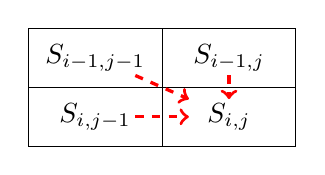
\begin{tikzpicture}[set style={{help lines}+=[dashed]}, xscale=1.7, yscale=0.75]

\draw (0,0) grid +(2,2);

\node  at  (0.5, 1.5) {$S_{i-1,j-1}$};
\node  at  (1.5, 0.5) {$S_{i,j}$};
\node  at  (0.5, 0.5) {$S_{i,j-1}$};
\node  at  (1.5, 1.5) {$S_{i-1,j}$};
\draw   [red,very thick,dashed,->]   (0.8,1.2) -- (1.2,0.8);
\draw   [red,very thick,dashed,->]   (1.5,1.2) -- (1.5,0.8);
\draw   [red,very thick,dashed,->]   (0.8,0.5) -- (1.2,0.5);

% -------- Fill numbers -----------
\end{tikzpicture} 
\end{center}


\end{overprint}

\end{columns}

\end{frame}
% Initiation------------------------------------------------
\begin{frame}
\frametitle{Example of Needleman-Wunsch (global alignment)}
Align $a=$GAC, $b=$ACG, using $\displaystyle d(x,y)= \begin{cases}1 & \textrm{if\ } x=y\\ -1 & \textrm{otherwise } \end{cases}$.

\begin{columns}

\column{0.4\textwidth}

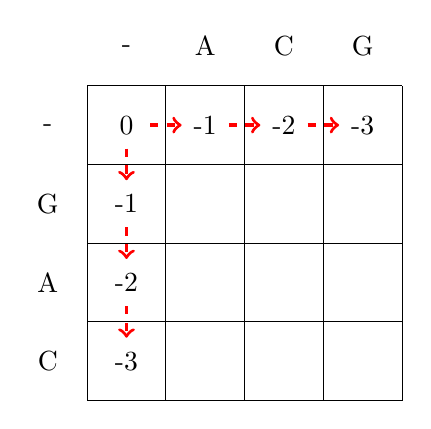
\begin{tikzpicture}[set style={{help lines}+=[dashed]}, xscale=1.0, yscale=1]

\draw (1,0) grid +(4,4);

\node  at  (0.5, 3.5) {-};
\node  at  (0.5, 2.5) {G};
\node  at  (0.5, 1.5) {A};
\node  at  (0.5, 0.5) {C};
\node  at  (1.5, 4.5) {-};
\node  at  (2.5, 4.5) {A};
\node  at  (3.5, 4.5) {C};
\node  at  (4.5, 4.5) {G};


\node  at  (1.5, 3.5) {0};
\node  at  (1.5, 2.5) {-1};
\node  at  (1.5, 1.5) {-2};
\node  at  (1.5, 0.5) {-3};
\node  at  (2.5, 3.5) {-1};
\node  at  (3.5, 3.5) {-2};
\node  at  (4.5, 3.5) {-3};

\draw   [red,very thick,dashed,->]   (1.5,3.2) -- (1.5,2.8);
\draw   [red,very thick,dashed,->]   (1.5,2.2) -- (1.5,1.8);
\draw   [red,very thick,dashed,->]   (1.5,1.2) -- (1.5,0.8);
\draw   [red,very thick,dashed,->]   (1.8,3.5) -- (2.2,3.5);
\draw   [red,very thick,dashed,->]   (2.8,3.5) -- (3.2,3.5);
\draw   [red,very thick,dashed,->]   (3.8,3.5) -- (4.2,3.5);


% -------- Fill numbers -----------
\end{tikzpicture} 

\column{0.6\textwidth}
\begin{align*}
 S_{0,0} =& 0, \\
S_{i,0} =& -1 \cdot i \ \textrm{for all}\ i, \\
S_{0,j} =&  -1 \cdot j\ \textrm{for all}\ j 
\end{align*}

\end{columns}

\end{frame}

%------------------------------------------------
\begin{frame}
\frametitle{Example of Needleman-Wunsch (global alignment)}
Align $a=$GAC, $b=$ACG, using $\displaystyle d(x,y)= \begin{cases}1 & \textrm{if\ } x=y\\ -1 & \textrm{otherwise } \end{cases}$.

\begin{columns}

\column{0.4\textwidth}

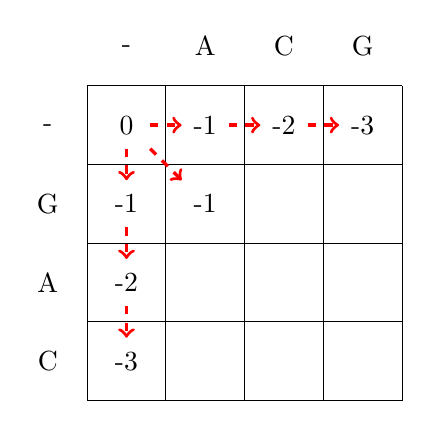
\begin{tikzpicture}[set style={{help lines}+=[dashed]}, xscale=1.0, yscale=1]

\draw (1,0) grid +(4,4);

\node  at  (0.5, 3.5) {-};
\node  at  (0.5, 2.5) {G};
\node  at  (0.5, 1.5) {A};
\node  at  (0.5, 0.5) {C};
\node  at  (1.5, 4.5) {-};
\node  at  (2.5, 4.5) {A};
\node  at  (3.5, 4.5) {C};
\node  at  (4.5, 4.5) {G};


\node  at  (1.5, 3.5) {0};
\node  at  (1.5, 2.5) {-1};
\node  at  (1.5, 1.5) {-2};
\node  at  (1.5, 0.5) {-3};
\node  at  (2.5, 3.5) {-1};
\node  at  (3.5, 3.5) {-2};
\node  at  (4.5, 3.5) {-3};

\draw   [red,very thick,dashed,->]   (1.5,3.2) -- (1.5,2.8);
\draw   [red,very thick,dashed,->]   (1.5,2.2) -- (1.5,1.8);
\draw   [red,very thick,dashed,->]   (1.5,1.2) -- (1.5,0.8);
\draw   [red,very thick,dashed,->]   (1.8,3.5) -- (2.2,3.5);
\draw   [red,very thick,dashed,->]   (2.8,3.5) -- (3.2,3.5);
\draw   [red,very thick,dashed,->]   (3.8,3.5) -- (4.2,3.5);

\draw   [red,very thick,dashed,->]   (1.8,3.2) -- (2.2,2.8);
\node  at  (2.5, 2.5) {-1};


% -------- Fill numbers -----------
\end{tikzpicture} 

\column{0.6\textwidth}
\[ 
S_{1,1}=\max
\begin{cases}
   S_{0,0} + d(G,A) & = 0 + -1 = -1\\
   S_{0,1} + d(G,-) & = -1 + -1 = -2\\
   S_{1,0} + d(-,A) & = -1 + -1 = -2
\end{cases}
\]

\end{columns}

\end{frame}

%------------------------------------------------
\begin{frame}
\frametitle{Example of Needleman-Wunsch (global alignment)}
Align $a=$GAC, $b=$ACG, using $\displaystyle d(x,y)= \begin{cases}1 & \textrm{if\ } x=y\\ -1 & \textrm{otherwise } \end{cases}$.

\begin{columns}

\column{0.4\textwidth}

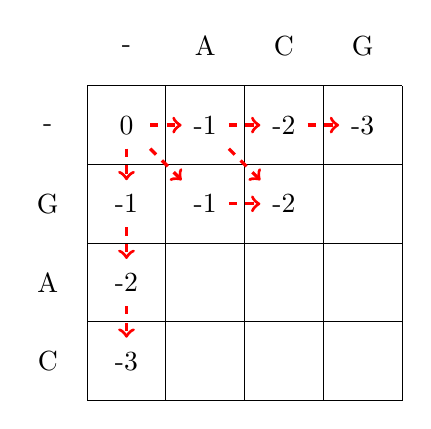
\begin{tikzpicture}[set style={{help lines}+=[dashed]}, xscale=1.0, yscale=1]

\draw (1,0) grid +(4,4);

\node  at  (0.5, 3.5) {-};
\node  at  (0.5, 2.5) {G};
\node  at  (0.5, 1.5) {A};
\node  at  (0.5, 0.5) {C};
\node  at  (1.5, 4.5) {-};
\node  at  (2.5, 4.5) {A};
\node  at  (3.5, 4.5) {C};
\node  at  (4.5, 4.5) {G};


\node  at  (1.5, 3.5) {0};
\node  at  (1.5, 2.5) {-1};
\node  at  (1.5, 1.5) {-2};
\node  at  (1.5, 0.5) {-3};
\node  at  (2.5, 3.5) {-1};
\node  at  (3.5, 3.5) {-2};
\node  at  (4.5, 3.5) {-3};

\draw   [red,very thick,dashed,->]   (1.5,3.2) -- (1.5,2.8);
\draw   [red,very thick,dashed,->]   (1.5,2.2) -- (1.5,1.8);
\draw   [red,very thick,dashed,->]   (1.5,1.2) -- (1.5,0.8);
\draw   [red,very thick,dashed,->]   (1.8,3.5) -- (2.2,3.5);
\draw   [red,very thick,dashed,->]   (2.8,3.5) -- (3.2,3.5);
\draw   [red,very thick,dashed,->]   (3.8,3.5) -- (4.2,3.5);

\draw   [red,very thick,dashed,->]   (1.8,3.2) -- (2.2,2.8);
\node  at  (2.5, 2.5) {-1};

\draw   [red,very thick,dashed,->]   (2.8,3.2) -- (3.2,2.8);
\draw   [red,very thick,dashed,->]   (2.8,2.5) -- (3.2,2.5);
%\draw   [red,very thick,dashed,->]   (3.5,3.2) -- (3.5,2.8);
\node  at  (3.5, 2.5) {-2};


% -------- Fill numbers -----------
\end{tikzpicture} 

\column{0.6\textwidth}
\[ 
S_{1,2}=\max
\begin{cases}
   S_{0,1} + d(G,C) & = -1 + -1 = -2\\
   S_{0,2} + d(G,-) & = -2 + -1 = -3\\
   S_{1,1} + d(-,C) & = -1 + -1 = -2
\end{cases}
\]

\end{columns}

\end{frame}

%------------------------------------------------
\begin{frame}
\frametitle{Example of Needleman-Wunsch (global alignment)}
Align $a=$GAC, $b=$ACG, using $\displaystyle d(x,y)= \begin{cases}1 & \textrm{if\ } x=y\\ -1 & \textrm{otherwise } \end{cases}$.

\begin{columns}

\column{0.4\textwidth}

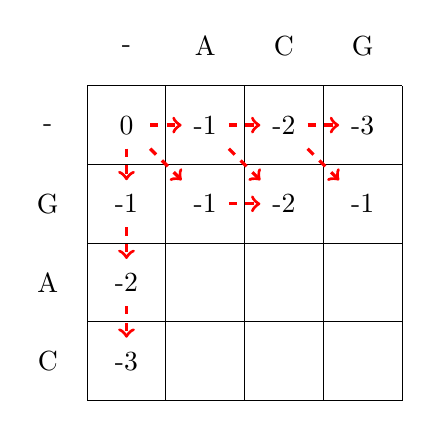
\begin{tikzpicture}[set style={{help lines}+=[dashed]}, xscale=1.0, yscale=1]

\draw (1,0) grid +(4,4);

\node  at  (0.5, 3.5) {-};
\node  at  (0.5, 2.5) {G};
\node  at  (0.5, 1.5) {A};
\node  at  (0.5, 0.5) {C};
\node  at  (1.5, 4.5) {-};
\node  at  (2.5, 4.5) {A};
\node  at  (3.5, 4.5) {C};
\node  at  (4.5, 4.5) {G};


\node  at  (1.5, 3.5) {0};
\node  at  (1.5, 2.5) {-1};
\node  at  (1.5, 1.5) {-2};
\node  at  (1.5, 0.5) {-3};
\node  at  (2.5, 3.5) {-1};
\node  at  (3.5, 3.5) {-2};
\node  at  (4.5, 3.5) {-3};

\draw   [red,very thick,dashed,->]   (1.5,3.2) -- (1.5,2.8);
\draw   [red,very thick,dashed,->]   (1.5,2.2) -- (1.5,1.8);
\draw   [red,very thick,dashed,->]   (1.5,1.2) -- (1.5,0.8);
\draw   [red,very thick,dashed,->]   (1.8,3.5) -- (2.2,3.5);
\draw   [red,very thick,dashed,->]   (2.8,3.5) -- (3.2,3.5);
\draw   [red,very thick,dashed,->]   (3.8,3.5) -- (4.2,3.5);

\draw   [red,very thick,dashed,->]   (1.8,3.2) -- (2.2,2.8);
\node  at  (2.5, 2.5) {-1};

\draw   [red,very thick,dashed,->]   (2.8,3.2) -- (3.2,2.8);
\draw   [red,very thick,dashed,->]   (2.8,2.5) -- (3.2,2.5);
%\draw   [red,very thick,dashed,->]   (3.5,3.2) -- (3.5,2.8);
\node  at  (3.5, 2.5) {-2};

\draw   [red,very thick,dashed,->]   (3.8,3.2) -- (4.2,2.8);
%\draw   [red,very thick,dashed,->]   (3.8,2.5) -- (4.2,2.5);
%\draw   [red,very thick,dashed,->]   (4.5,3.2) -- (4.5,2.8);
\node  at  (4.5, 2.5) {-1};


% -------- Fill numbers -----------
\end{tikzpicture} 

\column{0.6\textwidth}
\[ 
S_{1,3}=\max
\begin{cases}
   S_{0,2} + d(G,G) & = -2 + 1 = -1\\
   S_{0,3} + d(G,-) & = -3 + -1 = -4\\
   S_{1,2} + d(-,G) & = -2 + -1 = -3
\end{cases}
\]

\end{columns}

\end{frame}

% 2nd row ------------------------------------------------
\begin{frame}
\frametitle{Example of Needleman-Wunsch (global alignment)}
Align $a=$GAC, $b=$ACG, using $\displaystyle d(x,y)= \begin{cases}1 & \textrm{if\ } x=y\\ -1 & \textrm{otherwise } \end{cases}$.

\begin{columns}

\column{0.4\textwidth}

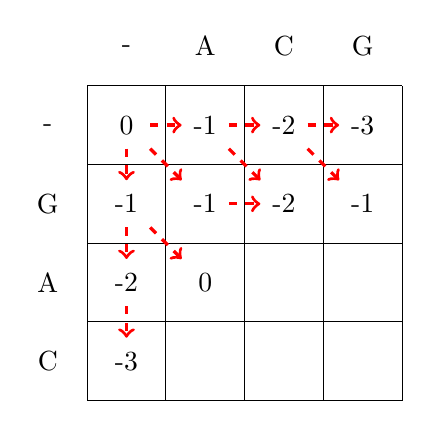
\begin{tikzpicture}[set style={{help lines}+=[dashed]}, xscale=1.0, yscale=1]

\draw (1,0) grid +(4,4);

\node  at  (0.5, 3.5) {-};
\node  at  (0.5, 2.5) {G};
\node  at  (0.5, 1.5) {A};
\node  at  (0.5, 0.5) {C};
\node  at  (1.5, 4.5) {-};
\node  at  (2.5, 4.5) {A};
\node  at  (3.5, 4.5) {C};
\node  at  (4.5, 4.5) {G};


\node  at  (1.5, 3.5) {0};
\node  at  (1.5, 2.5) {-1};
\node  at  (1.5, 1.5) {-2};
\node  at  (1.5, 0.5) {-3};
\node  at  (2.5, 3.5) {-1};
\node  at  (3.5, 3.5) {-2};
\node  at  (4.5, 3.5) {-3};

\draw   [red,very thick,dashed,->]   (1.5,3.2) -- (1.5,2.8);
\draw   [red,very thick,dashed,->]   (1.5,2.2) -- (1.5,1.8);
\draw   [red,very thick,dashed,->]   (1.5,1.2) -- (1.5,0.8);
\draw   [red,very thick,dashed,->]   (1.8,3.5) -- (2.2,3.5);
\draw   [red,very thick,dashed,->]   (2.8,3.5) -- (3.2,3.5);
\draw   [red,very thick,dashed,->]   (3.8,3.5) -- (4.2,3.5);

\draw   [red,very thick,dashed,->]   (1.8,3.2) -- (2.2,2.8);
\node  at  (2.5, 2.5) {-1};

\draw   [red,very thick,dashed,->]   (2.8,3.2) -- (3.2,2.8);
\draw   [red,very thick,dashed,->]   (2.8,2.5) -- (3.2,2.5);
%\draw   [red,very thick,dashed,->]   (3.5,3.2) -- (3.5,2.8);
\node  at  (3.5, 2.5) {-2};

\draw   [red,very thick,dashed,->]   (3.8,3.2) -- (4.2,2.8);
%\draw   [red,very thick,dashed,->]   (3.8,2.5) -- (4.2,2.5);
%\draw   [red,very thick,dashed,->]   (4.5,3.2) -- (4.5,2.8);
\node  at  (4.5, 2.5) {-1};

% Second row
\draw   [red,very thick,dashed,->]   (1.8,2.2) -- (2.2,1.8);
\node  at  (2.5, 1.5) {0};

% -------- Fill numbers -----------
\end{tikzpicture} 

\column{0.6\textwidth}
\[ 
S_{2,1}=\max
\begin{cases}
   S_{1,0} + d(A,A) & = -1 + 1 = 0\\
   S_{1,1} + d(A,-) & = -1 + -1 = -2\\
   S_{2,0} + d(-,A) & = -2 + -1 = -3
\end{cases}
\]

\end{columns}

\end{frame}

% 2nd row, 2 col ------------------------------------------------
\begin{frame}
\frametitle{Example of Needleman-Wunsch (global alignment)}
Align $a=$GAC, $b=$ACG, using $\displaystyle d(x,y)= \begin{cases}1 & \textrm{if\ } x=y\\ -1 & \textrm{otherwise } \end{cases}$.

\begin{columns}

\column{0.4\textwidth}

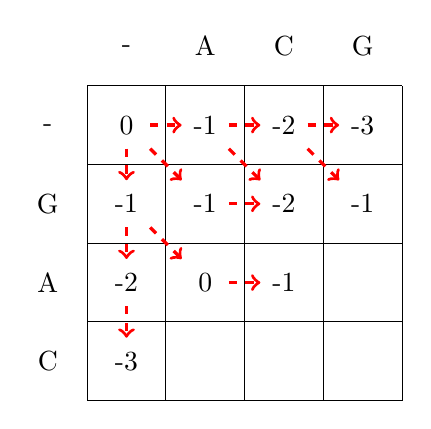
\begin{tikzpicture}[set style={{help lines}+=[dashed]}, xscale=1.0, yscale=1]

\draw (1,0) grid +(4,4);

\node  at  (0.5, 3.5) {-};
\node  at  (0.5, 2.5) {G};
\node  at  (0.5, 1.5) {A};
\node  at  (0.5, 0.5) {C};
\node  at  (1.5, 4.5) {-};
\node  at  (2.5, 4.5) {A};
\node  at  (3.5, 4.5) {C};
\node  at  (4.5, 4.5) {G};


\node  at  (1.5, 3.5) {0};
\node  at  (1.5, 2.5) {-1};
\node  at  (1.5, 1.5) {-2};
\node  at  (1.5, 0.5) {-3};
\node  at  (2.5, 3.5) {-1};
\node  at  (3.5, 3.5) {-2};
\node  at  (4.5, 3.5) {-3};

\draw   [red,very thick,dashed,->]   (1.5,3.2) -- (1.5,2.8);
\draw   [red,very thick,dashed,->]   (1.5,2.2) -- (1.5,1.8);
\draw   [red,very thick,dashed,->]   (1.5,1.2) -- (1.5,0.8);
\draw   [red,very thick,dashed,->]   (1.8,3.5) -- (2.2,3.5);
\draw   [red,very thick,dashed,->]   (2.8,3.5) -- (3.2,3.5);
\draw   [red,very thick,dashed,->]   (3.8,3.5) -- (4.2,3.5);

\draw   [red,very thick,dashed,->]   (1.8,3.2) -- (2.2,2.8);
\node  at  (2.5, 2.5) {-1};

\draw   [red,very thick,dashed,->]   (2.8,3.2) -- (3.2,2.8);
\draw   [red,very thick,dashed,->]   (2.8,2.5) -- (3.2,2.5);
%\draw   [red,very thick,dashed,->]   (3.5,3.2) -- (3.5,2.8);
\node  at  (3.5, 2.5) {-2};

\draw   [red,very thick,dashed,->]   (3.8,3.2) -- (4.2,2.8);
%\draw   [red,very thick,dashed,->]   (3.8,2.5) -- (4.2,2.5);
%\draw   [red,very thick,dashed,->]   (4.5,3.2) -- (4.5,2.8);
\node  at  (4.5, 2.5) {-1};

% Second row
\draw   [red,very thick,dashed,->]   (1.8,2.2) -- (2.2,1.8);
\node  at  (2.5, 1.5) {0};
\draw   [red,very thick,dashed,->]   (2.8,1.5) -- (3.2,1.5);
\node  at  (3.5, 1.5) {-1};

% -------- Fill numbers -----------
\end{tikzpicture} 

\column{0.6\textwidth}
\[ 
S_{2,2}=\max
\begin{cases}
   S_{1,1} + d(A,C) & = -1 + -1 = -2\\
   S_{1,2} + d(A,-) & = -2 + -1 = -3\\
   S_{2,1} + d(-,C) & = 0 + -1 = -1
\end{cases}
\]

\end{columns}

\end{frame}

% 2nd row, 3 col ------------------------------------------------
\begin{frame}
\frametitle{Example of Needleman-Wunsch (global alignment)}
Align $a=$GAC, $b=$ACG, using $\displaystyle d(x,y)= \begin{cases}1 & \textrm{if\ } x=y\\ -1 & \textrm{otherwise } \end{cases}$.

\begin{columns}

\column{0.4\textwidth}

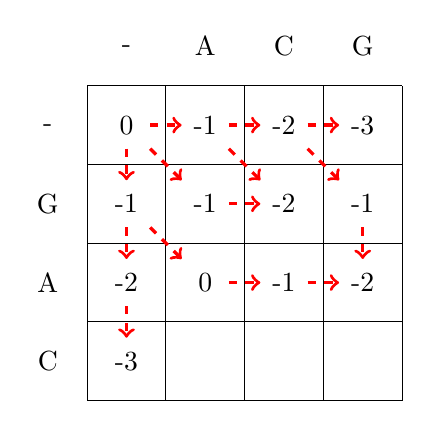
\begin{tikzpicture}[set style={{help lines}+=[dashed]}, xscale=1.0, yscale=1]

\draw (1,0) grid +(4,4);

\node  at  (0.5, 3.5) {-};
\node  at  (0.5, 2.5) {G};
\node  at  (0.5, 1.5) {A};
\node  at  (0.5, 0.5) {C};
\node  at  (1.5, 4.5) {-};
\node  at  (2.5, 4.5) {A};
\node  at  (3.5, 4.5) {C};
\node  at  (4.5, 4.5) {G};


\node  at  (1.5, 3.5) {0};
\node  at  (1.5, 2.5) {-1};
\node  at  (1.5, 1.5) {-2};
\node  at  (1.5, 0.5) {-3};
\node  at  (2.5, 3.5) {-1};
\node  at  (3.5, 3.5) {-2};
\node  at  (4.5, 3.5) {-3};

\draw   [red,very thick,dashed,->]   (1.5,3.2) -- (1.5,2.8);
\draw   [red,very thick,dashed,->]   (1.5,2.2) -- (1.5,1.8);
\draw   [red,very thick,dashed,->]   (1.5,1.2) -- (1.5,0.8);
\draw   [red,very thick,dashed,->]   (1.8,3.5) -- (2.2,3.5);
\draw   [red,very thick,dashed,->]   (2.8,3.5) -- (3.2,3.5);
\draw   [red,very thick,dashed,->]   (3.8,3.5) -- (4.2,3.5);

\draw   [red,very thick,dashed,->]   (1.8,3.2) -- (2.2,2.8);
\node  at  (2.5, 2.5) {-1};

\draw   [red,very thick,dashed,->]   (2.8,3.2) -- (3.2,2.8);
\draw   [red,very thick,dashed,->]   (2.8,2.5) -- (3.2,2.5);
%\draw   [red,very thick,dashed,->]   (3.5,3.2) -- (3.5,2.8);
\node  at  (3.5, 2.5) {-2};

\draw   [red,very thick,dashed,->]   (3.8,3.2) -- (4.2,2.8);
%\draw   [red,very thick,dashed,->]   (3.8,2.5) -- (4.2,2.5);
%\draw   [red,very thick,dashed,->]   (4.5,3.2) -- (4.5,2.8);
\node  at  (4.5, 2.5) {-1};

% Second row
\draw   [red,very thick,dashed,->]   (1.8,2.2) -- (2.2,1.8);
\node  at  (2.5, 1.5) {0};
\draw   [red,very thick,dashed,->]   (2.8,1.5) -- (3.2,1.5);
\node  at  (3.5, 1.5) {-1};
\draw   [red,very thick,dashed,->]   (3.8,1.5) -- (4.2,1.5);
\draw   [red,very thick,dashed,->]   (4.5,2.2) -- (4.5,1.8);
\node  at  (4.5, 1.5) {-2};

% -------- Fill numbers -----------
\end{tikzpicture} 

\column{0.6\textwidth}
\[ 
S_{2,3}=\max
\begin{cases}
   S_{1,2} + d(A,G) & = -2 + -1 = -3\\
   S_{1,3} + d(A,-) & = -1 + -1 = -2\\
   S_{2,2} + d(-,G) & = -1 + -1 = -2
\end{cases}
\]

\end{columns}

\end{frame}

% 3rd row, 1 col ------------------------------------------------
\begin{frame}
\frametitle{Example of Needleman-Wunsch (global alignment)}
Align $a=$GAC, $b=$ACG, using $\displaystyle d(x,y)= \begin{cases}1 & \textrm{if\ } x=y\\ -1 & \textrm{otherwise } \end{cases}$.

\begin{columns}

\column{0.4\textwidth}

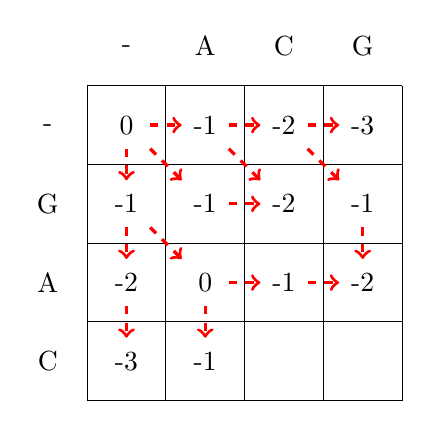
\begin{tikzpicture}[set style={{help lines}+=[dashed]}, xscale=1.0, yscale=1]

\draw (1,0) grid +(4,4);

\node  at  (0.5, 3.5) {-};
\node  at  (0.5, 2.5) {G};
\node  at  (0.5, 1.5) {A};
\node  at  (0.5, 0.5) {C};
\node  at  (1.5, 4.5) {-};
\node  at  (2.5, 4.5) {A};
\node  at  (3.5, 4.5) {C};
\node  at  (4.5, 4.5) {G};


\node  at  (1.5, 3.5) {0};
\node  at  (1.5, 2.5) {-1};
\node  at  (1.5, 1.5) {-2};
\node  at  (1.5, 0.5) {-3};
\node  at  (2.5, 3.5) {-1};
\node  at  (3.5, 3.5) {-2};
\node  at  (4.5, 3.5) {-3};

\draw   [red,very thick,dashed,->]   (1.5,3.2) -- (1.5,2.8);
\draw   [red,very thick,dashed,->]   (1.5,2.2) -- (1.5,1.8);
\draw   [red,very thick,dashed,->]   (1.5,1.2) -- (1.5,0.8);
\draw   [red,very thick,dashed,->]   (1.8,3.5) -- (2.2,3.5);
\draw   [red,very thick,dashed,->]   (2.8,3.5) -- (3.2,3.5);
\draw   [red,very thick,dashed,->]   (3.8,3.5) -- (4.2,3.5);

\draw   [red,very thick,dashed,->]   (1.8,3.2) -- (2.2,2.8);
\node  at  (2.5, 2.5) {-1};

\draw   [red,very thick,dashed,->]   (2.8,3.2) -- (3.2,2.8);
\draw   [red,very thick,dashed,->]   (2.8,2.5) -- (3.2,2.5);
%\draw   [red,very thick,dashed,->]   (3.5,3.2) -- (3.5,2.8);
\node  at  (3.5, 2.5) {-2};

\draw   [red,very thick,dashed,->]   (3.8,3.2) -- (4.2,2.8);
%\draw   [red,very thick,dashed,->]   (3.8,2.5) -- (4.2,2.5);
%\draw   [red,very thick,dashed,->]   (4.5,3.2) -- (4.5,2.8);
\node  at  (4.5, 2.5) {-1};

% Second row
\draw   [red,very thick,dashed,->]   (1.8,2.2) -- (2.2,1.8);
\node  at  (2.5, 1.5) {0};
\draw   [red,very thick,dashed,->]   (2.8,1.5) -- (3.2,1.5);
\node  at  (3.5, 1.5) {-1};
\draw   [red,very thick,dashed,->]   (3.8,1.5) -- (4.2,1.5);
\draw   [red,very thick,dashed,->]   (4.5,2.2) -- (4.5,1.8);
\node  at  (4.5, 1.5) {-2};

% Third row
%\draw   [red,very thick,dashed,->]   (1.8,1.2) -- (2.2,0.8);
\draw   [red,very thick,dashed,->]   (2.5,1.2) -- (2.5,0.8);
\node  at  (2.5, 0.5) {-1};


% -------- Fill numbers -----------
\end{tikzpicture} 

\column{0.6\textwidth}
\[ 
S_{3,1}=\max
\begin{cases}
   S_{2,0} + d(C,A) & = -2 + -1 = -3\\
   S_{2,1} + d(C,-) & = 0 + -1 = -1\\
   S_{3,0} + d(-,A) & = -3 + -1 = -4
\end{cases}
\]

\end{columns}

\end{frame}


% 3rd row, 2 col ------------------------------------------------
\begin{frame}
\frametitle{Example of Needleman-Wunsch (global alignment)}
Align $a=$GAC, $b=$ACG, using $\displaystyle d(x,y)= \begin{cases}1 & \textrm{if\ } x=y\\ -1 & \textrm{otherwise } \end{cases}$.

\begin{columns}

\column{0.4\textwidth}

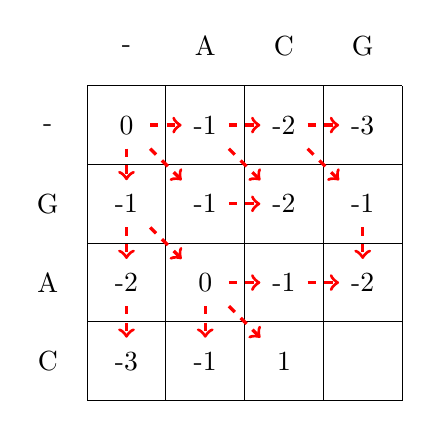
\begin{tikzpicture}[set style={{help lines}+=[dashed]}, xscale=1.0, yscale=1]

\draw (1,0) grid +(4,4);

\node  at  (0.5, 3.5) {-};
\node  at  (0.5, 2.5) {G};
\node  at  (0.5, 1.5) {A};
\node  at  (0.5, 0.5) {C};
\node  at  (1.5, 4.5) {-};
\node  at  (2.5, 4.5) {A};
\node  at  (3.5, 4.5) {C};
\node  at  (4.5, 4.5) {G};


\node  at  (1.5, 3.5) {0};
\node  at  (1.5, 2.5) {-1};
\node  at  (1.5, 1.5) {-2};
\node  at  (1.5, 0.5) {-3};
\node  at  (2.5, 3.5) {-1};
\node  at  (3.5, 3.5) {-2};
\node  at  (4.5, 3.5) {-3};

\draw   [red,very thick,dashed,->]   (1.5,3.2) -- (1.5,2.8);
\draw   [red,very thick,dashed,->]   (1.5,2.2) -- (1.5,1.8);
\draw   [red,very thick,dashed,->]   (1.5,1.2) -- (1.5,0.8);
\draw   [red,very thick,dashed,->]   (1.8,3.5) -- (2.2,3.5);
\draw   [red,very thick,dashed,->]   (2.8,3.5) -- (3.2,3.5);
\draw   [red,very thick,dashed,->]   (3.8,3.5) -- (4.2,3.5);

\draw   [red,very thick,dashed,->]   (1.8,3.2) -- (2.2,2.8);
\node  at  (2.5, 2.5) {-1};

\draw   [red,very thick,dashed,->]   (2.8,3.2) -- (3.2,2.8);
\draw   [red,very thick,dashed,->]   (2.8,2.5) -- (3.2,2.5);
%\draw   [red,very thick,dashed,->]   (3.5,3.2) -- (3.5,2.8);
\node  at  (3.5, 2.5) {-2};

\draw   [red,very thick,dashed,->]   (3.8,3.2) -- (4.2,2.8);
%\draw   [red,very thick,dashed,->]   (3.8,2.5) -- (4.2,2.5);
%\draw   [red,very thick,dashed,->]   (4.5,3.2) -- (4.5,2.8);
\node  at  (4.5, 2.5) {-1};

% Second row
\draw   [red,very thick,dashed,->]   (1.8,2.2) -- (2.2,1.8);
\node  at  (2.5, 1.5) {0};
\draw   [red,very thick,dashed,->]   (2.8,1.5) -- (3.2,1.5);
\node  at  (3.5, 1.5) {-1};
\draw   [red,very thick,dashed,->]   (3.8,1.5) -- (4.2,1.5);
\draw   [red,very thick,dashed,->]   (4.5,2.2) -- (4.5,1.8);
\node  at  (4.5, 1.5) {-2};

% Third row
%\draw   [red,very thick,dashed,->]   (1.8,1.2) -- (2.2,0.8);
\draw   [red,very thick,dashed,->]   (2.5,1.2) -- (2.5,0.8);
\node  at  (2.5, 0.5) {-1};
\draw   [red,very thick,dashed,->]   (2.8,1.2) -- (3.2,0.8);
%\draw   [red,very thick,dashed,->]   (3.5,1.2) -- (3.5,0.8);
\node  at  (3.5, 0.5) {1};


% -------- Fill numbers -----------
\end{tikzpicture} 

\column{0.6\textwidth}
\[ 
S_{3,2}=\max
\begin{cases}
   S_{2,1} + d(C,C) & = 0 + 1 = +1\\
   S_{2,2} + d(C,-) & = -1 + -1 = -2\\
   S_{3,1} + d(-,C) & = -1 + -1 = -2
\end{cases}
\]

\end{columns}

\end{frame}

% 3rd row, 3 col ------------------------------------------------
\begin{frame}
\frametitle{Example of Needleman-Wunsch (global alignment)}
Align $a=$GAC, $b=$ACG, using $\displaystyle d(x,y)= \begin{cases}1 & \textrm{if\ } x=y\\ -1 & \textrm{otherwise } \end{cases}$.

\begin{columns}

\column{0.4\textwidth}

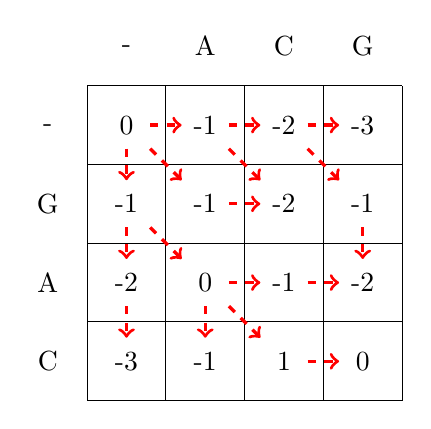
\begin{tikzpicture}[set style={{help lines}+=[dashed]}, xscale=1.0, yscale=1]

\draw (1,0) grid +(4,4);

\node  at  (0.5, 3.5) {-};
\node  at  (0.5, 2.5) {G};
\node  at  (0.5, 1.5) {A};
\node  at  (0.5, 0.5) {C};
\node  at  (1.5, 4.5) {-};
\node  at  (2.5, 4.5) {A};
\node  at  (3.5, 4.5) {C};
\node  at  (4.5, 4.5) {G};


\node  at  (1.5, 3.5) {0};
\node  at  (1.5, 2.5) {-1};
\node  at  (1.5, 1.5) {-2};
\node  at  (1.5, 0.5) {-3};
\node  at  (2.5, 3.5) {-1};
\node  at  (3.5, 3.5) {-2};
\node  at  (4.5, 3.5) {-3};

\draw   [red,very thick,dashed,->]   (1.5,3.2) -- (1.5,2.8);
\draw   [red,very thick,dashed,->]   (1.5,2.2) -- (1.5,1.8);
\draw   [red,very thick,dashed,->]   (1.5,1.2) -- (1.5,0.8);
\draw   [red,very thick,dashed,->]   (1.8,3.5) -- (2.2,3.5);
\draw   [red,very thick,dashed,->]   (2.8,3.5) -- (3.2,3.5);
\draw   [red,very thick,dashed,->]   (3.8,3.5) -- (4.2,3.5);

\draw   [red,very thick,dashed,->]   (1.8,3.2) -- (2.2,2.8);
\node  at  (2.5, 2.5) {-1};

\draw   [red,very thick,dashed,->]   (2.8,3.2) -- (3.2,2.8);
\draw   [red,very thick,dashed,->]   (2.8,2.5) -- (3.2,2.5);
%\draw   [red,very thick,dashed,->]   (3.5,3.2) -- (3.5,2.8);
\node  at  (3.5, 2.5) {-2};

\draw   [red,very thick,dashed,->]   (3.8,3.2) -- (4.2,2.8);
%\draw   [red,very thick,dashed,->]   (3.8,2.5) -- (4.2,2.5);
%\draw   [red,very thick,dashed,->]   (4.5,3.2) -- (4.5,2.8);
\node  at  (4.5, 2.5) {-1};

% Second row
\draw   [red,very thick,dashed,->]   (1.8,2.2) -- (2.2,1.8);
\node  at  (2.5, 1.5) {0};
\draw   [red,very thick,dashed,->]   (2.8,1.5) -- (3.2,1.5);
\node  at  (3.5, 1.5) {-1};
\draw   [red,very thick,dashed,->]   (3.8,1.5) -- (4.2,1.5);
\draw   [red,very thick,dashed,->]   (4.5,2.2) -- (4.5,1.8);
\node  at  (4.5, 1.5) {-2};

% Third row
%\draw   [red,very thick,dashed,->]   (1.8,1.2) -- (2.2,0.8);
\draw   [red,very thick,dashed,->]   (2.5,1.2) -- (2.5,0.8);
\node  at  (2.5, 0.5) {-1};
\draw   [red,very thick,dashed,->]   (2.8,1.2) -- (3.2,0.8);
%\draw   [red,very thick,dashed,->]   (3.5,1.2) -- (3.5,0.8);
\node  at  (3.5, 0.5) {1};
%\draw   [red,very thick,dashed,->]   (3.8,1.2) -- (4.2,0.8);
%\draw   [red,very thick,dashed,->]   (4.5,1.2) -- (4.5,0.8);
\draw   [red,very thick,dashed,->]   (3.8,0.5) -- (4.2,0.5);
\node  at  (4.5, 0.5) {0};


% -------- Fill numbers -----------
\end{tikzpicture} 

\column{0.6\textwidth}
\[ 
S_{3,3}=\max
\begin{cases}
   S_{2,2} + d(C,G) & = -1 + -1 = -2\\
   S_{2,3} + d(C,-) & = -2 + -1 = -3\\
   S_{3,2} + d(-,G) & = 1 + -1 = 0
\end{cases}
\]

\end{columns}

\end{frame}

% Backptr ------------------------------------------------
\begin{frame}
\frametitle{Example of Needleman-Wunsch (global alignment)}
Align $a=$GAC, $b=$ACG, using $\displaystyle d(x,y)= \begin{cases}1 & \textrm{if\ } x=y\\ -1 & \textrm{otherwise } \end{cases}$.

\begin{columns}

\column{0.4\textwidth}

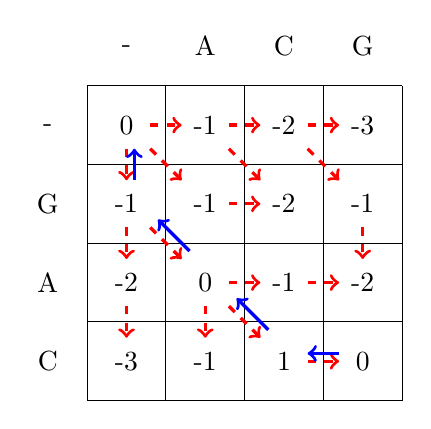
\begin{tikzpicture}[set style={{help lines}+=[dashed]}, xscale=1.0, yscale=1]

\draw (1,0) grid +(4,4);

\node  at  (0.5, 3.5) {-};
\node  at  (0.5, 2.5) {G};
\node  at  (0.5, 1.5) {A};
\node  at  (0.5, 0.5) {C};
\node  at  (1.5, 4.5) {-};
\node  at  (2.5, 4.5) {A};
\node  at  (3.5, 4.5) {C};
\node  at  (4.5, 4.5) {G};


\node  at  (1.5, 3.5) {0};
\node  at  (1.5, 2.5) {-1};
\node  at  (1.5, 1.5) {-2};
\node  at  (1.5, 0.5) {-3};
\node  at  (2.5, 3.5) {-1};
\node  at  (3.5, 3.5) {-2};
\node  at  (4.5, 3.5) {-3};

\draw   [red,very thick,dashed,->]   (1.5,3.2) -- (1.5,2.8);
\draw   [blue,very thick,<-]   (1.6,3.2) -- (1.6,2.8);
\draw   [red,very thick,dashed,->]   (1.5,2.2) -- (1.5,1.8);
\draw   [red,very thick,dashed,->]   (1.5,1.2) -- (1.5,0.8);
\draw   [red,very thick,dashed,->]   (1.8,3.5) -- (2.2,3.5);
\draw   [red,very thick,dashed,->]   (2.8,3.5) -- (3.2,3.5);
\draw   [red,very thick,dashed,->]   (3.8,3.5) -- (4.2,3.5);

\draw   [red,very thick,dashed,->]   (1.8,3.2) -- (2.2,2.8);
\node  at  (2.5, 2.5) {-1};

\draw   [red,very thick,dashed,->]   (2.8,3.2) -- (3.2,2.8);
\draw   [red,very thick,dashed,->]   (2.8,2.5) -- (3.2,2.5);
%\draw   [red,very thick,dashed,->]   (3.5,3.2) -- (3.5,2.8);
\node  at  (3.5, 2.5) {-2};

\draw   [red,very thick,dashed,->]   (3.8,3.2) -- (4.2,2.8);
%\draw   [red,very thick,dashed,->]   (3.8,2.5) -- (4.2,2.5);
%\draw   [red,very thick,dashed,->]   (4.5,3.2) -- (4.5,2.8);
\node  at  (4.5, 2.5) {-1};

% Second row
\draw   [red,very thick,dashed,->]   (1.8,2.2) -- (2.2,1.8);
\draw   [blue,very thick,<-]   (1.9,2.3) -- (2.3,1.9);
\node  at  (2.5, 1.5) {0};
\draw   [red,very thick,dashed,->]   (2.8,1.5) -- (3.2,1.5);
\node  at  (3.5, 1.5) {-1};
\draw   [red,very thick,dashed,->]   (3.8,1.5) -- (4.2,1.5);
\draw   [red,very thick,dashed,->]   (4.5,2.2) -- (4.5,1.8);
\node  at  (4.5, 1.5) {-2};

% Third row
%\draw   [red,very thick,dashed,->]   (1.8,1.2) -- (2.2,0.8);
\draw   [red,very thick,dashed,->]   (2.5,1.2) -- (2.5,0.8);
\node  at  (2.5, 0.5) {-1};
\draw   [red,very thick,dashed,->]   (2.8,1.2) -- (3.2,0.8);
\draw   [blue,very thick,<-]   (2.9,1.3) -- (3.3,0.9);
%\draw   [red,very thick,dashed,->]   (3.5,1.2) -- (3.5,0.8);
\node  at  (3.5, 0.5) {1};
%\draw   [red,very thick,dashed,->]   (3.8,1.2) -- (4.2,0.8);
%\draw   [red,very thick,dashed,->]   (4.5,1.2) -- (4.5,0.8);
\draw   [red,very thick,dashed,->]   (3.8,0.5) -- (4.2,0.5);
\draw   [blue,very thick,<-]   (3.8,0.6) -- (4.2,0.6);
\node  at  (4.5, 0.5) {0};


% -------- Fill numbers -----------
\end{tikzpicture} 

\column{0.6\textwidth}

Optimal score given by $S_{3,3}=0$.\\[2ex]

An optimal alignment can be found by \textcolor{blue}{back tracing} (-,G), (C,C), (A,A), (G,-) i.e.\\[2ex]
{\verb GGAC-\\
  -ACG}
\end{columns}

\end{frame}

% Larger example ------------------------------------------------
\begin{frame}
\frametitle{Larger Example of Needleman-Wunsch (global alignment)}
$a=$TGCATTA $b=$GCATTAC when $\displaystyle d(x,y)= \begin{cases}3 & \textrm{if\ } x=y\\-2 & \textrm{if\ } x= \textrm{``-'' or\ } y=\textrm{``-''}\\  -1 & \textrm{otherwise } \end{cases}$.

\begin{columns}

\column{0.5\textwidth}

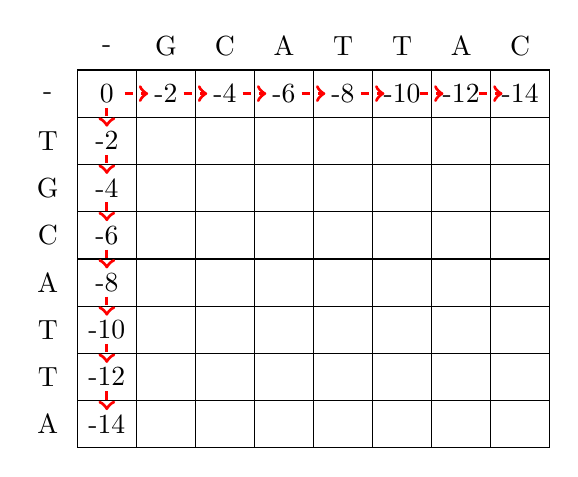
\begin{tikzpicture}[set style={{help lines}+=[dashed]}, xscale=0.75, yscale=0.6]

\draw (1,0) grid +(8,8);

\node  at  (0.5, 7.5) {-};
\node  at  (0.5, 6.5) {T};
\node  at  (0.5, 5.5) {G};
\node  at  (0.5, 4.5) {C};
\node  at  (0.5, 3.5) {A};
\node  at  (0.5, 2.5) {T};
\node  at  (0.5, 1.5) {T};
\node  at  (0.5, 0.5) {A};
\node  at  (1.5, 8.5) {-};
\node  at  (2.5, 8.5) {G};
\node  at  (3.5, 8.5) {C};
\node  at  (4.5, 8.5) {A};
\node  at  (5.5, 8.5) {T};
\node  at  (6.5, 8.5) {T};
\node  at  (7.5, 8.5) {A};
\node  at  (8.5, 8.5) {C};

% First col
\node  at  (1.5, 7.5) {0};
\node  at  (1.5, 6.5) {-2};
\node  at  (1.5, 5.5) {-4};
\node  at  (1.5, 4.5) {-6};
\node  at  (1.5, 3.5) {-8};
\node  at  (1.5, 2.5) {-10};
\node  at  (1.5, 1.5) {-12};
\node  at  (1.5, 0.5) {-14};

\draw   [red,very thick,dashed,->]   (1.5,7.2) -- (1.5,6.8);
\draw   [red,very thick,dashed,->]   (1.5,6.2) -- (1.5,5.8);
\draw   [red,very thick,dashed,->]   (1.5,5.2) -- (1.5,4.8);
\draw   [red,very thick,dashed,->]   (1.5,4.2) -- (1.5,3.8);
\draw   [red,very thick,dashed,->]   (1.5,3.2) -- (1.5,2.8);
\draw   [red,very thick,dashed,->]   (1.5,2.2) -- (1.5,1.8);
\draw   [red,very thick,dashed,->]   (1.5,1.2) -- (1.5,0.8);

% First row
\node  at  (2.5, 7.5) {-2};
\node  at  (3.5, 7.5) {-4};
\node  at  (4.5, 7.5) {-6};
\node  at  (5.5, 7.5) {-8};
\node  at  (6.5, 7.5) {-10};
\node  at  (7.5, 7.5) {-12};
\node  at  (8.5, 7.5) {-14};

\draw   [red,very thick,dashed,->]   (1.8,7.5) -- (2.2,7.5);
\draw   [red,very thick,dashed,->]   (2.8,7.5) -- (3.2,7.5);
\draw   [red,very thick,dashed,->]   (3.8,7.5) -- (4.2,7.5);
\draw   [red,very thick,dashed,->]   (4.8,7.5) -- (5.2,7.5);
\draw   [red,very thick,dashed,->]   (5.8,7.5) -- (6.2,7.5);
\draw   [red,very thick,dashed,->]   (6.8,7.5) -- (7.2,7.5);
\draw   [red,very thick,dashed,->]   (7.8,7.5) -- (8.2,7.5);

\end{tikzpicture} 

\column{0.6\textwidth}

Initiate matrix with gap penalties
\end{columns}

\end{frame}

% Larger example ------------------------------------------------
\begin{frame}
\frametitle{Larger Example of Needleman-Wunsch (global alignment)}
$a=$TGCATTA $b=$GCATTAC when $\displaystyle d(x,y)= \begin{cases}3 & \textrm{if\ } x=y\\-2 & \textrm{if\ } x= \textrm{``-'' or\ } y=\textrm{``-''}\\  -1 & \textrm{otherwise } \end{cases}$.

\begin{columns}

\column{0.5\textwidth}

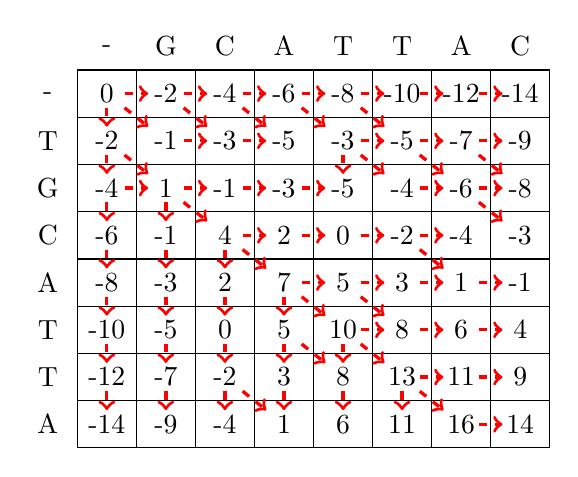
\begin{tikzpicture}[set style={{help lines}+=[dashed]}, xscale=0.75, yscale=0.6]

\draw (1,0) grid +(8,8);

\node  at  (0.5, 7.5) {-};
\node  at  (0.5, 6.5) {T};
\node  at  (0.5, 5.5) {G};
\node  at  (0.5, 4.5) {C};
\node  at  (0.5, 3.5) {A};
\node  at  (0.5, 2.5) {T};
\node  at  (0.5, 1.5) {T};
\node  at  (0.5, 0.5) {A};
\node  at  (1.5, 8.5) {-};
\node  at  (2.5, 8.5) {G};
\node  at  (3.5, 8.5) {C};
\node  at  (4.5, 8.5) {A};
\node  at  (5.5, 8.5) {T};
\node  at  (6.5, 8.5) {T};
\node  at  (7.5, 8.5) {A};
\node  at  (8.5, 8.5) {C};

% First col
\node  at  (1.5, 7.5) {0};
\node  at  (1.5, 6.5) {-2};
\node  at  (1.5, 5.5) {-4};
\node  at  (1.5, 4.5) {-6};
\node  at  (1.5, 3.5) {-8};
\node  at  (1.5, 2.5) {-10};
\node  at  (1.5, 1.5) {-12};
\node  at  (1.5, 0.5) {-14};

\draw   [red,very thick,dashed,->]   (1.5,7.2) -- (1.5,6.8);
%\draw   [blue,very thick,<-]         (1.7,7.2) -- (1.7,6.8);
\draw   [red,very thick,dashed,->]   (1.5,6.2) -- (1.5,5.8);
\draw   [red,very thick,dashed,->]   (1.5,5.2) -- (1.5,4.8);
\draw   [red,very thick,dashed,->]   (1.5,4.2) -- (1.5,3.8);
\draw   [red,very thick,dashed,->]   (1.5,3.2) -- (1.5,2.8);
\draw   [red,very thick,dashed,->]   (1.5,2.2) -- (1.5,1.8);
\draw   [red,very thick,dashed,->]   (1.5,1.2) -- (1.5,0.8);

% First row
\node  at  (2.5, 7.5) {-2};
\node  at  (3.5, 7.5) {-4};
\node  at  (4.5, 7.5) {-6};
\node  at  (5.5, 7.5) {-8};
\node  at  (6.5, 7.5) {-10};
\node  at  (7.5, 7.5) {-12};
\node  at  (8.5, 7.5) {-14};

\draw   [red,very thick,dashed,->]   (1.8,7.5) -- (2.2,7.5);
\draw   [red,very thick,dashed,->]   (2.8,7.5) -- (3.2,7.5);
\draw   [red,very thick,dashed,->]   (3.8,7.5) -- (4.2,7.5);
\draw   [red,very thick,dashed,->]   (4.8,7.5) -- (5.2,7.5);
\draw   [red,very thick,dashed,->]   (5.8,7.5) -- (6.2,7.5);
\draw   [red,very thick,dashed,->]   (6.8,7.5) -- (7.2,7.5);
\draw   [red,very thick,dashed,->]   (7.8,7.5) -- (8.2,7.5);

% Second row
\node  at  (2.5, 6.5) {-1};
\node  at  (3.5, 6.5) {-3};
\node  at  (4.5, 6.5) {-5};
\node  at  (5.5, 6.5) {-3};
\node  at  (6.5, 6.5) {-5};
\node  at  (7.5, 6.5) {-7};
\node  at  (8.5, 6.5) {-9};

%\draw   [red,very thick,dashed,->]   (1.8,6.5) -- (2.2,6.5);
\draw   [red,very thick,dashed,->]   (2.8,6.5) -- (3.2,6.5);
\draw   [red,very thick,dashed,->]   (3.8,6.5) -- (4.2,6.5);
%\draw   [red,very thick,dashed,->]   (4.8,6.5) -- (5.2,6.5);
\draw   [red,very thick,dashed,->]   (5.8,6.5) -- (6.2,6.5);
\draw   [red,very thick,dashed,->]   (6.8,6.5) -- (7.2,6.5);
\draw   [red,very thick,dashed,->]   (7.8,6.5) -- (8.2,6.5);

\draw   [red,very thick,dashed,->]   (1.8,7.2) -- (2.2,6.8);
\draw   [red,very thick,dashed,->]   (2.8,7.2) -- (3.2,6.8);
\draw   [red,very thick,dashed,->]   (3.8,7.2) -- (4.2,6.8);
\draw   [red,very thick,dashed,->]   (4.8,7.2) -- (5.2,6.8);
\draw   [red,very thick,dashed,->]   (5.8,7.2) -- (6.2,6.8);
%\draw   [red,very thick,dashed,->]   (6.8,7.2) -- (7.2,6.8);
%\draw   [red,very thick,dashed,->]   (7.8,7.2) -- (8.2,6.8);

% Third row
\node  at  (2.5, 5.5) {1};
\node  at  (3.5, 5.5) {-1};
\node  at  (4.5, 5.5) {-3};
\node  at  (5.5, 5.5) {-5};
\node  at  (6.5, 5.5) {-4};
\node  at  (7.5, 5.5) {-6};
\node  at  (8.5, 5.5) {-8};

\draw   [red,very thick,dashed,->]   (1.8,5.5) -- (2.2,5.5);
\draw   [red,very thick,dashed,->]   (2.8,5.5) -- (3.2,5.5);
\draw   [red,very thick,dashed,->]   (3.8,5.5) -- (4.2,5.5);
\draw   [red,very thick,dashed,->]   (4.8,5.5) -- (5.2,5.5);
%\draw   [red,very thick,dashed,->]   (5.8,5.5) -- (6.2,5.5);
\draw   [red,very thick,dashed,->]   (6.8,5.5) -- (7.2,5.5);
\draw   [red,very thick,dashed,->]   (7.8,5.5) -- (8.2,5.5);

\draw   [red,very thick,dashed,->]   (1.8,6.2) -- (2.2,5.8);
%\draw   [blue,very thick,<-]         (1.9,6.3) -- (2.3,5.9);
%\draw   [red,very thick,dashed,->]   (2.8,6.2) -- (3.2,5.8);
%\draw   [red,very thick,dashed,->]   (3.8,6.2) -- (4.2,5.8);
%\draw   [red,very thick,dashed,->]   (4.8,6.2) -- (5.2,5.8);
\draw   [red,very thick,dashed,->]   (5.8,6.2) -- (6.2,5.8);
\draw   [red,very thick,dashed,->]   (6.8,6.2) -- (7.2,5.8);
\draw   [red,very thick,dashed,->]   (7.8,6.2) -- (8.2,5.8);

\draw   [red,very thick,dashed,->]   (5.5,6.2) -- (5.5,5.8);

% Forth row
\node  at  (2.5, 4.5) {-1};
\node  at  (3.5, 4.5) {4};
\node  at  (4.5, 4.5) {2};
\node  at  (5.5, 4.5) {0};
\node  at  (6.5, 4.5) {-2};
\node  at  (7.5, 4.5) {-4};
\node  at  (8.5, 4.5) {-3};

%\draw   [red,very thick,dashed,->]   (1.8,4.5) -- (2.2,4.5);
%\draw   [red,very thick,dashed,->]   (2.8,4.5) -- (3.2,4.5);
\draw   [red,very thick,dashed,->]   (3.8,4.5) -- (4.2,4.5);
\draw   [red,very thick,dashed,->]   (4.8,4.5) -- (5.2,4.5);
\draw   [red,very thick,dashed,->]   (5.8,4.5) -- (6.2,4.5);
\draw   [red,very thick,dashed,->]   (6.8,4.5) -- (7.2,4.5);
%\draw   [red,very thick,dashed,->]   (7.8,4.5) -- (8.2,4.5);

%\draw   [red,very thick,dashed,->]   (1.8,5.2) -- (2.2,4.8);
\draw   [red,very thick,dashed,->]   (2.8,5.2) -- (3.2,4.8);
%\draw   [blue,very thick,<-]         (2.9,5.3) -- (3.3,4.9);
%\draw   [red,very thick,dashed,->]   (3.8,5.2) -- (4.2,4.8);
%\draw   [red,very thick,dashed,->]   (4.8,5.2) -- (5.2,4.8);
%\draw   [red,very thick,dashed,->]   (5.8,5.2) -- (6.2,4.8);
%\draw   [red,very thick,dashed,->]   (6.8,5.2) -- (7.2,4.8);
\draw   [red,very thick,dashed,->]   (7.8,5.2) -- (8.2,4.8);

\draw   [red,very thick,dashed,->]   (2.5,5.2) -- (2.5,4.8);


% Fifth row
\node  at  (2.5, 3.5) {-3};
\node  at  (3.5, 3.5) {2};
\node  at  (4.5, 3.5) {7};
\node  at  (5.5, 3.5) {5};
\node  at  (6.5, 3.5) {3};
\node  at  (7.5, 3.5) {1};
\node  at  (8.5, 3.5) {-1};

%\draw   [red,very thick,dashed,->]   (1.8,3.5) -- (2.2,3.5);
%\draw   [red,very thick,dashed,->]   (2.8,3.5) -- (3.2,3.5);
%\draw   [red,very thick,dashed,->]   (3.8,3.5) -- (4.2,3.5);
\draw   [red,very thick,dashed,->]   (4.8,3.5) -- (5.2,3.5);
\draw   [red,very thick,dashed,->]   (5.8,3.5) -- (6.2,3.5);
\draw   [red,very thick,dashed,->]   (6.8,3.5) -- (7.2,3.5);
\draw   [red,very thick,dashed,->]   (7.8,3.5) -- (8.2,3.5);

%\draw   [red,very thick,dashed,->]   (1.8,4.2) -- (2.2,3.8);
%\draw   [red,very thick,dashed,->]   (2.8,4.2) -- (3.2,3.8);
\draw   [red,very thick,dashed,->]   (3.8,4.2) -- (4.2,3.8);
%\draw   [blue,very thick,<-]         (3.9,4.3) -- (4.3,3.9);
%\draw   [red,very thick,dashed,->]   (4.8,4.2) -- (5.2,3.8);
%\draw   [red,very thick,dashed,->]   (5.8,4.2) -- (6.2,3.8);
\draw   [red,very thick,dashed,->]   (6.8,4.2) -- (7.2,3.8);
%\draw   [red,very thick,dashed,->]   (7.8,4.2) -- (8.2,3.8);

\draw   [red,very thick,dashed,->]   (2.5,4.2) -- (2.5,3.8);
\draw   [red,very thick,dashed,->]   (3.5,4.2) -- (3.5,3.8);

% Sixth row
\node  at  (2.5, 2.5) {-5};
\node  at  (3.5, 2.5) {0};
\node  at  (4.5, 2.5) {5};
\node  at  (5.5, 2.5) {10};
\node  at  (6.5, 2.5) {8};
\node  at  (7.5, 2.5) {6};
\node  at  (8.5, 2.5) {4};

\draw   [red,very thick,dashed,->]   (5.8,2.5) -- (6.2,2.5);
\draw   [red,very thick,dashed,->]   (6.8,2.5) -- (7.2,2.5);
\draw   [red,very thick,dashed,->]   (7.8,2.5) -- (8.2,2.5);

%\draw   [red,very thick,dashed,->]   (1.8,3.2) -- (2.2,2.8);
%\draw   [red,very thick,dashed,->]   (2.8,3.2) -- (3.2,2.8);
%\draw   [red,very thick,dashed,->]   (3.8,3.2) -- (4.2,2.8);
\draw   [red,very thick,dashed,->]   (4.8,3.2) -- (5.2,2.8);
%\draw   [blue,very thick,<-]         (4.9,3.3) -- (5.3,2.9);
\draw   [red,very thick,dashed,->]   (5.8,3.2) -- (6.2,2.8);
%\draw   [red,very thick,dashed,->]   (6.8,3.2) -- (7.2,2.8);
%\draw   [red,very thick,dashed,->]   (7.8,3.2) -- (8.2,2.8);

\draw   [red,very thick,dashed,->]   (2.5,3.2) -- (2.5,2.8);
\draw   [red,very thick,dashed,->]   (3.5,3.2) -- (3.5,2.8);
\draw   [red,very thick,dashed,->]   (4.5,3.2) -- (4.5,2.8);

% Seventh row
\node  at  (2.5, 1.5) {-7};
\node  at  (3.5, 1.5) {-2};
\node  at  (4.5, 1.5) {3};
\node  at  (5.5, 1.5) {8};
\node  at  (6.5, 1.5) {13};
\node  at  (7.5, 1.5) {11};
\node  at  (8.5, 1.5) {9};

\draw   [red,very thick,dashed,->]   (6.8,1.5) -- (7.2,1.5);
\draw   [red,very thick,dashed,->]   (7.8,1.5) -- (8.2,1.5);

%\draw   [red,very thick,dashed,->]   (1.8,2.2) -- (2.2,1.8);
%\draw   [red,very thick,dashed,->]   (2.8,2.2) -- (3.2,1.8);
%\draw   [red,very thick,dashed,->]   (3.8,2.2) -- (4.2,1.8);
\draw   [red,very thick,dashed,->]   (4.8,2.2) -- (5.2,1.8);
\draw   [red,very thick,dashed,->]   (5.8,2.2) -- (6.2,1.8);
%\draw   [blue,very thick,<-]         (5.9,2.3) -- (6.3,1.9);
%\draw   [red,very thick,dashed,->]   (6.8,2.2) -- (7.2,1.8);
%\draw   [red,very thick,dashed,->]   (7.8,2.2) -- (8.2,1.8);

\draw   [red,very thick,dashed,->]   (2.5,2.2) -- (2.5,1.8);
\draw   [red,very thick,dashed,->]   (3.5,2.2) -- (3.5,1.8);
\draw   [red,very thick,dashed,->]   (4.5,2.2) -- (4.5,1.8);
\draw   [red,very thick,dashed,->]   (5.5,2.2) -- (5.5,1.8);

% Eighth row
\node  at  (2.5, 0.5) {-9};
\node  at  (3.5, 0.5) {-4};
\node  at  (4.5, 0.5) {1};
\node  at  (5.5, 0.5) {6};
\node  at  (6.5, 0.5) {11};
\node  at  (7.5, 0.5) {16};
\node  at  (8.5, 0.5) {14};

\draw   [red,very thick,dashed,->]   (7.8,0.5) -- (8.2,0.5);
%\draw   [blue,very thick,<-]         (7.8,0.7) -- (8.2,0.7);

%\draw   [red,very thick,dashed,->]   (1.8,1.2) -- (2.2,0.8);
%\draw   [red,very thick,dashed,->]   (2.8,1.2) -- (3.2,0.8);
\draw   [red,very thick,dashed,->]   (3.8,1.2) -- (4.2,0.8);
%\draw   [red,very thick,dashed,->]   (4.8,1.2) -- (5.2,0.8);
%\draw   [red,very thick,dashed,->]   (5.8,1.2) -- (6.2,0.8);
\draw   [red,very thick,dashed,->]   (6.8,1.2) -- (7.2,0.8);
%\draw   [blue,very thick,<-]         (6.9,1.3) -- (7.3,0.9);
%\draw   [red,very thick,dashed,->]   (7.8,1.2) -- (8.2,0.8);

\draw   [red,very thick,dashed,->]   (2.5,1.2) -- (2.5,0.8);
\draw   [red,very thick,dashed,->]   (3.5,1.2) -- (3.5,0.8);
\draw   [red,very thick,dashed,->]   (4.5,1.2) -- (4.5,0.8);
\draw   [red,very thick,dashed,->]   (5.5,1.2) -- (5.5,0.8);
\draw   [red,very thick,dashed,->]   (6.5,1.2) -- (6.5,0.8);
% -------- Fill numbers -----------
\end{tikzpicture} 

\column{0.6\textwidth}

Fill in the rest of the matrix
\end{columns}

\end{frame}

% Larger example ------------------------------------------------
\begin{frame}
\frametitle{Larger Example of Needleman-Wunsch (global alignment)}
$a=$TGCATTA $b=$GCATTAC when $\displaystyle d(x,y)= \begin{cases}3 & \textrm{if\ } x=y\\-2 & \textrm{if\ } x= \textrm{``-'' or\ } y=\textrm{``-''}\\  -1 & \textrm{otherwise } \end{cases}$.

\begin{columns}

\column{0.5\textwidth}

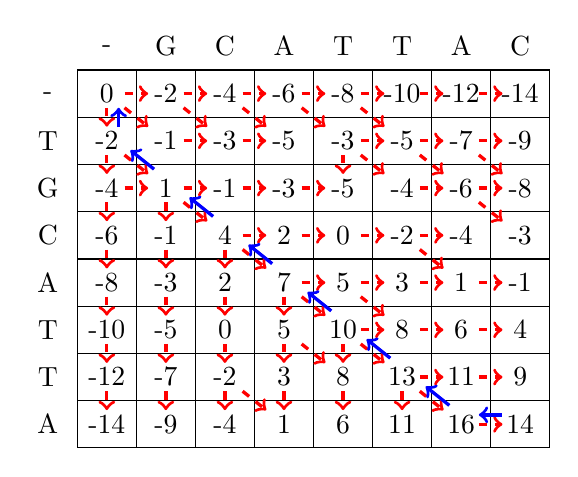
\begin{tikzpicture}[set style={{help lines}+=[dashed]}, xscale=0.75, yscale=0.6]

\draw (1,0) grid +(8,8);

\node  at  (0.5, 7.5) {-};
\node  at  (0.5, 6.5) {T};
\node  at  (0.5, 5.5) {G};
\node  at  (0.5, 4.5) {C};
\node  at  (0.5, 3.5) {A};
\node  at  (0.5, 2.5) {T};
\node  at  (0.5, 1.5) {T};
\node  at  (0.5, 0.5) {A};
\node  at  (1.5, 8.5) {-};
\node  at  (2.5, 8.5) {G};
\node  at  (3.5, 8.5) {C};
\node  at  (4.5, 8.5) {A};
\node  at  (5.5, 8.5) {T};
\node  at  (6.5, 8.5) {T};
\node  at  (7.5, 8.5) {A};
\node  at  (8.5, 8.5) {C};

% First col
\node  at  (1.5, 7.5) {0};
\node  at  (1.5, 6.5) {-2};
\node  at  (1.5, 5.5) {-4};
\node  at  (1.5, 4.5) {-6};
\node  at  (1.5, 3.5) {-8};
\node  at  (1.5, 2.5) {-10};
\node  at  (1.5, 1.5) {-12};
\node  at  (1.5, 0.5) {-14};

\draw   [red,very thick,dashed,->]   (1.5,7.2) -- (1.5,6.8);
\draw   [blue,very thick,<-]         (1.7,7.2) -- (1.7,6.8);
\draw   [red,very thick,dashed,->]   (1.5,6.2) -- (1.5,5.8);
\draw   [red,very thick,dashed,->]   (1.5,5.2) -- (1.5,4.8);
\draw   [red,very thick,dashed,->]   (1.5,4.2) -- (1.5,3.8);
\draw   [red,very thick,dashed,->]   (1.5,3.2) -- (1.5,2.8);
%\draw   [blue,very thick,<-]   (1.6,3.2) -- (1.6,2.8);
\draw   [red,very thick,dashed,->]   (1.5,2.2) -- (1.5,1.8);
\draw   [red,very thick,dashed,->]   (1.5,1.2) -- (1.5,0.8);

% First row
\node  at  (2.5, 7.5) {-2};
\node  at  (3.5, 7.5) {-4};
\node  at  (4.5, 7.5) {-6};
\node  at  (5.5, 7.5) {-8};
\node  at  (6.5, 7.5) {-10};
\node  at  (7.5, 7.5) {-12};
\node  at  (8.5, 7.5) {-14};

\draw   [red,very thick,dashed,->]   (1.8,7.5) -- (2.2,7.5);
\draw   [red,very thick,dashed,->]   (2.8,7.5) -- (3.2,7.5);
\draw   [red,very thick,dashed,->]   (3.8,7.5) -- (4.2,7.5);
\draw   [red,very thick,dashed,->]   (4.8,7.5) -- (5.2,7.5);
\draw   [red,very thick,dashed,->]   (5.8,7.5) -- (6.2,7.5);
\draw   [red,very thick,dashed,->]   (6.8,7.5) -- (7.2,7.5);
\draw   [red,very thick,dashed,->]   (7.8,7.5) -- (8.2,7.5);

% Second row
\node  at  (2.5, 6.5) {-1};
\node  at  (3.5, 6.5) {-3};
\node  at  (4.5, 6.5) {-5};
\node  at  (5.5, 6.5) {-3};
\node  at  (6.5, 6.5) {-5};
\node  at  (7.5, 6.5) {-7};
\node  at  (8.5, 6.5) {-9};

%\draw   [red,very thick,dashed,->]   (1.8,6.5) -- (2.2,6.5);
\draw   [red,very thick,dashed,->]   (2.8,6.5) -- (3.2,6.5);
\draw   [red,very thick,dashed,->]   (3.8,6.5) -- (4.2,6.5);
%\draw   [red,very thick,dashed,->]   (4.8,6.5) -- (5.2,6.5);
\draw   [red,very thick,dashed,->]   (5.8,6.5) -- (6.2,6.5);
\draw   [red,very thick,dashed,->]   (6.8,6.5) -- (7.2,6.5);
\draw   [red,very thick,dashed,->]   (7.8,6.5) -- (8.2,6.5);

\draw   [red,very thick,dashed,->]   (1.8,7.2) -- (2.2,6.8);
\draw   [red,very thick,dashed,->]   (2.8,7.2) -- (3.2,6.8);
\draw   [red,very thick,dashed,->]   (3.8,7.2) -- (4.2,6.8);
\draw   [red,very thick,dashed,->]   (4.8,7.2) -- (5.2,6.8);
\draw   [red,very thick,dashed,->]   (5.8,7.2) -- (6.2,6.8);
%\draw   [red,very thick,dashed,->]   (6.8,7.2) -- (7.2,6.8);
%\draw   [red,very thick,dashed,->]   (7.8,7.2) -- (8.2,6.8);

% Third row
\node  at  (2.5, 5.5) {1};
\node  at  (3.5, 5.5) {-1};
\node  at  (4.5, 5.5) {-3};
\node  at  (5.5, 5.5) {-5};
\node  at  (6.5, 5.5) {-4};
\node  at  (7.5, 5.5) {-6};
\node  at  (8.5, 5.5) {-8};

\draw   [red,very thick,dashed,->]   (1.8,5.5) -- (2.2,5.5);
\draw   [red,very thick,dashed,->]   (2.8,5.5) -- (3.2,5.5);
\draw   [red,very thick,dashed,->]   (3.8,5.5) -- (4.2,5.5);
\draw   [red,very thick,dashed,->]   (4.8,5.5) -- (5.2,5.5);
%\draw   [red,very thick,dashed,->]   (5.8,5.5) -- (6.2,5.5);
\draw   [red,very thick,dashed,->]   (6.8,5.5) -- (7.2,5.5);
\draw   [red,very thick,dashed,->]   (7.8,5.5) -- (8.2,5.5);

\draw   [red,very thick,dashed,->]   (1.8,6.2) -- (2.2,5.8);
\draw   [blue,very thick,<-]         (1.9,6.3) -- (2.3,5.9);
%\draw   [red,very thick,dashed,->]   (2.8,6.2) -- (3.2,5.8);
%\draw   [red,very thick,dashed,->]   (3.8,6.2) -- (4.2,5.8);
%\draw   [red,very thick,dashed,->]   (4.8,6.2) -- (5.2,5.8);
\draw   [red,very thick,dashed,->]   (5.8,6.2) -- (6.2,5.8);
\draw   [red,very thick,dashed,->]   (6.8,6.2) -- (7.2,5.8);
\draw   [red,very thick,dashed,->]   (7.8,6.2) -- (8.2,5.8);

\draw   [red,very thick,dashed,->]   (5.5,6.2) -- (5.5,5.8);

% Forth row
\node  at  (2.5, 4.5) {-1};
\node  at  (3.5, 4.5) {4};
\node  at  (4.5, 4.5) {2};
\node  at  (5.5, 4.5) {0};
\node  at  (6.5, 4.5) {-2};
\node  at  (7.5, 4.5) {-4};
\node  at  (8.5, 4.5) {-3};

%\draw   [red,very thick,dashed,->]   (1.8,4.5) -- (2.2,4.5);
%\draw   [red,very thick,dashed,->]   (2.8,4.5) -- (3.2,4.5);
\draw   [red,very thick,dashed,->]   (3.8,4.5) -- (4.2,4.5);
\draw   [red,very thick,dashed,->]   (4.8,4.5) -- (5.2,4.5);
\draw   [red,very thick,dashed,->]   (5.8,4.5) -- (6.2,4.5);
\draw   [red,very thick,dashed,->]   (6.8,4.5) -- (7.2,4.5);
%\draw   [red,very thick,dashed,->]   (7.8,4.5) -- (8.2,4.5);

%\draw   [red,very thick,dashed,->]   (1.8,5.2) -- (2.2,4.8);
\draw   [red,very thick,dashed,->]   (2.8,5.2) -- (3.2,4.8);
\draw   [blue,very thick,<-]         (2.9,5.3) -- (3.3,4.9);
%\draw   [red,very thick,dashed,->]   (3.8,5.2) -- (4.2,4.8);
%\draw   [red,very thick,dashed,->]   (4.8,5.2) -- (5.2,4.8);
%\draw   [red,very thick,dashed,->]   (5.8,5.2) -- (6.2,4.8);
%\draw   [red,very thick,dashed,->]   (6.8,5.2) -- (7.2,4.8);
\draw   [red,very thick,dashed,->]   (7.8,5.2) -- (8.2,4.8);

\draw   [red,very thick,dashed,->]   (2.5,5.2) -- (2.5,4.8);


% Fifth row
\node  at  (2.5, 3.5) {-3};
\node  at  (3.5, 3.5) {2};
\node  at  (4.5, 3.5) {7};
\node  at  (5.5, 3.5) {5};
\node  at  (6.5, 3.5) {3};
\node  at  (7.5, 3.5) {1};
\node  at  (8.5, 3.5) {-1};

%\draw   [red,very thick,dashed,->]   (1.8,3.5) -- (2.2,3.5);
%\draw   [red,very thick,dashed,->]   (2.8,3.5) -- (3.2,3.5);
%\draw   [red,very thick,dashed,->]   (3.8,3.5) -- (4.2,3.5);
\draw   [red,very thick,dashed,->]   (4.8,3.5) -- (5.2,3.5);
\draw   [red,very thick,dashed,->]   (5.8,3.5) -- (6.2,3.5);
\draw   [red,very thick,dashed,->]   (6.8,3.5) -- (7.2,3.5);
\draw   [red,very thick,dashed,->]   (7.8,3.5) -- (8.2,3.5);

%\draw   [red,very thick,dashed,->]   (1.8,4.2) -- (2.2,3.8);
%\draw   [red,very thick,dashed,->]   (2.8,4.2) -- (3.2,3.8);
\draw   [red,very thick,dashed,->]   (3.8,4.2) -- (4.2,3.8);
\draw   [blue,very thick,<-]         (3.9,4.3) -- (4.3,3.9);
%\draw   [red,very thick,dashed,->]   (4.8,4.2) -- (5.2,3.8);
%\draw   [red,very thick,dashed,->]   (5.8,4.2) -- (6.2,3.8);
\draw   [red,very thick,dashed,->]   (6.8,4.2) -- (7.2,3.8);
%\draw   [red,very thick,dashed,->]   (7.8,4.2) -- (8.2,3.8);

\draw   [red,very thick,dashed,->]   (2.5,4.2) -- (2.5,3.8);
\draw   [red,very thick,dashed,->]   (3.5,4.2) -- (3.5,3.8);

% Sixth row
\node  at  (2.5, 2.5) {-5};
\node  at  (3.5, 2.5) {0};
\node  at  (4.5, 2.5) {5};
\node  at  (5.5, 2.5) {10};
\node  at  (6.5, 2.5) {8};
\node  at  (7.5, 2.5) {6};
\node  at  (8.5, 2.5) {4};

\draw   [red,very thick,dashed,->]   (5.8,2.5) -- (6.2,2.5);
\draw   [red,very thick,dashed,->]   (6.8,2.5) -- (7.2,2.5);
\draw   [red,very thick,dashed,->]   (7.8,2.5) -- (8.2,2.5);

%\draw   [red,very thick,dashed,->]   (1.8,3.2) -- (2.2,2.8);
%\draw   [red,very thick,dashed,->]   (2.8,3.2) -- (3.2,2.8);
%\draw   [red,very thick,dashed,->]   (3.8,3.2) -- (4.2,2.8);
\draw   [red,very thick,dashed,->]   (4.8,3.2) -- (5.2,2.8);
\draw   [blue,very thick,<-]         (4.9,3.3) -- (5.3,2.9);
\draw   [red,very thick,dashed,->]   (5.8,3.2) -- (6.2,2.8);
%\draw   [red,very thick,dashed,->]   (6.8,3.2) -- (7.2,2.8);
%\draw   [red,very thick,dashed,->]   (7.8,3.2) -- (8.2,2.8);

\draw   [red,very thick,dashed,->]   (2.5,3.2) -- (2.5,2.8);
\draw   [red,very thick,dashed,->]   (3.5,3.2) -- (3.5,2.8);
\draw   [red,very thick,dashed,->]   (4.5,3.2) -- (4.5,2.8);

% Seventh row
\node  at  (2.5, 1.5) {-7};
\node  at  (3.5, 1.5) {-2};
\node  at  (4.5, 1.5) {3};
\node  at  (5.5, 1.5) {8};
\node  at  (6.5, 1.5) {13};
\node  at  (7.5, 1.5) {11};
\node  at  (8.5, 1.5) {9};

\draw   [red,very thick,dashed,->]   (6.8,1.5) -- (7.2,1.5);
\draw   [red,very thick,dashed,->]   (7.8,1.5) -- (8.2,1.5);

%\draw   [red,very thick,dashed,->]   (1.8,2.2) -- (2.2,1.8);
%\draw   [red,very thick,dashed,->]   (2.8,2.2) -- (3.2,1.8);
%\draw   [red,very thick,dashed,->]   (3.8,2.2) -- (4.2,1.8);
\draw   [red,very thick,dashed,->]   (4.8,2.2) -- (5.2,1.8);
\draw   [red,very thick,dashed,->]   (5.8,2.2) -- (6.2,1.8);
\draw   [blue,very thick,<-]         (5.9,2.3) -- (6.3,1.9);
%\draw   [red,very thick,dashed,->]   (6.8,2.2) -- (7.2,1.8);
%\draw   [red,very thick,dashed,->]   (7.8,2.2) -- (8.2,1.8);

\draw   [red,very thick,dashed,->]   (2.5,2.2) -- (2.5,1.8);
\draw   [red,very thick,dashed,->]   (3.5,2.2) -- (3.5,1.8);
\draw   [red,very thick,dashed,->]   (4.5,2.2) -- (4.5,1.8);
\draw   [red,very thick,dashed,->]   (5.5,2.2) -- (5.5,1.8);

% Eighth row
\node  at  (2.5, 0.5) {-9};
\node  at  (3.5, 0.5) {-4};
\node  at  (4.5, 0.5) {1};
\node  at  (5.5, 0.5) {6};
\node  at  (6.5, 0.5) {11};
\node  at  (7.5, 0.5) {16};
\node  at  (8.5, 0.5) {14};

\draw   [red,very thick,dashed,->]   (7.8,0.5) -- (8.2,0.5);
\draw   [blue,very thick,<-]         (7.8,0.7) -- (8.2,0.7);

%\draw   [red,very thick,dashed,->]   (1.8,1.2) -- (2.2,0.8);
%\draw   [red,very thick,dashed,->]   (2.8,1.2) -- (3.2,0.8);
\draw   [red,very thick,dashed,->]   (3.8,1.2) -- (4.2,0.8);
%\draw   [red,very thick,dashed,->]   (4.8,1.2) -- (5.2,0.8);
%\draw   [red,very thick,dashed,->]   (5.8,1.2) -- (6.2,0.8);
\draw   [red,very thick,dashed,->]   (6.8,1.2) -- (7.2,0.8);
\draw   [blue,very thick,<-]         (6.9,1.3) -- (7.3,0.9);
%\draw   [red,very thick,dashed,->]   (7.8,1.2) -- (8.2,0.8);

\draw   [red,very thick,dashed,->]   (2.5,1.2) -- (2.5,0.8);
\draw   [red,very thick,dashed,->]   (3.5,1.2) -- (3.5,0.8);
\draw   [red,very thick,dashed,->]   (4.5,1.2) -- (4.5,0.8);
\draw   [red,very thick,dashed,->]   (5.5,1.2) -- (5.5,0.8);
\draw   [red,very thick,dashed,->]   (6.5,1.2) -- (6.5,0.8);
% -------- Fill numbers -----------
\end{tikzpicture} 

\column{0.6\textwidth}

Optimal score given by $S_{7,7}=14$.\\[2ex]

An optimal alignment can be found by \textcolor{blue}{back tracing} (-,C), (A,A), (T,T), (T,T), (A,A), (C,C), (G,G), (T,-) i.e.\\[2ex]
{\verb  TTGCATTA-\\
  -GCATTAC}
\end{columns}

\end{frame}


%------------------------------------------------
\begin{frame}
\frametitle{Smith-Waterman (local alignment)}
Given two sequences $a_1,\ldots,a_N$ and $b_1,\ldots,b_M$, a scoring function d(x,y), we can find an optimal {\em local} alignment by investigating the dynamic programming matrix of size (N+1,M+1), defined by

\begin{columns}

\column{0.6\textwidth}

\begin{align*}
 S_{0,0} =& 0, \\
S_{i,0} =& 0 \ \textrm{for all}\ i, \\
S_{0,j} =& 0 \ \textrm{for all}\ j 
\end{align*}
\[ S_{i,j}=\max
\begin{cases}
   S_{i-1,j-1} & + d(a_i,b_j)\\
   S_{i-1,j} & + d(a_i,-)\\
   S_{i,j-1} & + d(-,b_j)\\
   0\\
\end{cases}
\]

\column{0.4\textwidth}
The score of an optimal alignment is $\displaystyle \max_{i,j}S_{i,j}$

\begin{overprint}
\onslide<1>
\onslide<2>
\vspace{1cm}
\begin{center}
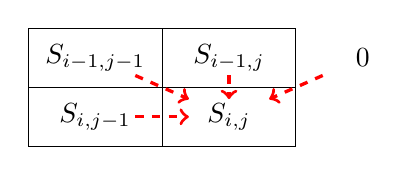
\begin{tikzpicture}[set style={{help lines}+=[dashed]}, xscale=1.7, yscale=0.75]

\draw (0,0) grid +(2,2);

\node  at  (0.5, 1.5) {$S_{i-1,j-1}$};
\node  at  (1.5, 0.5) {$S_{i,j}$};
\node  at  (0.5, 0.5) {$S_{i,j-1}$};
\node  at  (1.5, 1.5) {$S_{i-1,j}$};
\node  at  (2.5, 1.5) {$0$};
\draw   [red,very thick,dashed,->]   (0.8,1.2) -- (1.2,0.8);
\draw   [red,very thick,dashed,->]   (1.5,1.2) -- (1.5,0.8);
\draw   [red,very thick,dashed,->]   (0.8,0.5) -- (1.2,0.5);
\draw   [red,very thick,dashed,->]   (2.2,1.2) -- (1.8,0.8);

% -------- Fill numbers -----------
\end{tikzpicture} 
\end{center}


\end{overprint}

\end{columns}

\end{frame}

% Initiation------------------------------------------------
\begin{frame}
\frametitle{Example of Smith-Waterman (local alignment)}
Align $a=$GAC, $b=$ACG, using $\displaystyle d(x,y)= \begin{cases}1 & \textrm{if\ } x=y\\ -1 & \textrm{otherwise } \end{cases}$.

\begin{columns}

\column{0.4\textwidth}

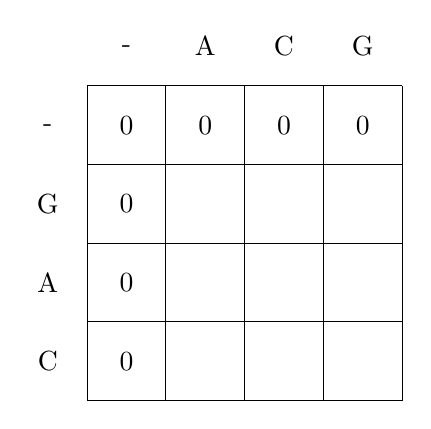
\begin{tikzpicture}[set style={{help lines}+=[dashed]}, xscale=1.0, yscale=1]

\draw (1,0) grid +(4,4);

\node  at  (0.5, 3.5) {-};
\node  at  (0.5, 2.5) {G};
\node  at  (0.5, 1.5) {A};
\node  at  (0.5, 0.5) {C};
\node  at  (1.5, 4.5) {-};
\node  at  (2.5, 4.5) {A};
\node  at  (3.5, 4.5) {C};
\node  at  (4.5, 4.5) {G};


\node  at  (1.5, 3.5) {0};
\node  at  (1.5, 2.5) {0};
\node  at  (1.5, 1.5) {0};
\node  at  (1.5, 0.5) {0};
\node  at  (2.5, 3.5) {0};
\node  at  (3.5, 3.5) {0};
\node  at  (4.5, 3.5) {0};


% -------- Fill numbers -----------
\end{tikzpicture} 

\column{0.6\textwidth}
\begin{align*}
 S_{0,0} =& 0, \\
S_{i,0} =& 0 \ \textrm{for all}\ i, \\
S_{0,j} =&  0 \cdot j\ \textrm{for all}\ j 
\end{align*}

\end{columns}

\end{frame}


% 3rd row, 3 col ------------------------------------------------
\begin{frame}
\frametitle{Example of Smith-Waterman (local alignment)}
Align $a=$GAC, $b=$ACG, using $\displaystyle d(x,y)= \begin{cases}1 & \textrm{if\ } x=y\\ -1 & \textrm{otherwise } \end{cases}$.

\begin{columns}

\column{0.4\textwidth}

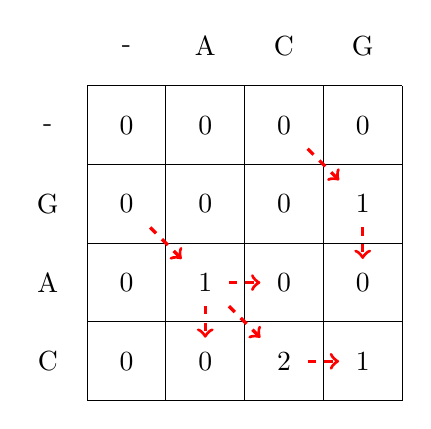
\begin{tikzpicture}[set style={{help lines}+=[dashed]}, xscale=1.0, yscale=1]

\draw (1,0) grid +(4,4);

\node  at  (0.5, 3.5) {-};
\node  at  (0.5, 2.5) {G};
\node  at  (0.5, 1.5) {A};
\node  at  (0.5, 0.5) {C};
\node  at  (1.5, 4.5) {-};
\node  at  (2.5, 4.5) {A};
\node  at  (3.5, 4.5) {C};
\node  at  (4.5, 4.5) {G};


\node  at  (1.5, 3.5) {0};
\node  at  (1.5, 2.5) {0};
\node  at  (1.5, 1.5) {0};
\node  at  (1.5, 0.5) {0};
\node  at  (2.5, 3.5) {0};
\node  at  (3.5, 3.5) {0};
\node  at  (4.5, 3.5) {0};

\node  at  (2.5, 2.5) {0};
\node  at  (3.5, 2.5) {0};

\draw   [red,very thick,dashed,->]   (3.8,3.2) -- (4.2,2.8);
%\draw   [red,very thick,dashed,->]   (3.8,2.5) -- (4.2,2.5);
%\draw   [red,very thick,dashed,->]   (4.5,3.2) -- (4.5,2.8);
\node  at  (4.5, 2.5) {1};

% Second row
\draw   [red,very thick,dashed,->]   (1.8,2.2) -- (2.2,1.8);
\node  at  (2.5, 1.5) {1};
\draw   [red,very thick,dashed,->]   (2.8,1.5) -- (3.2,1.5);
\node  at  (3.5, 1.5) {0};
%\draw   [red,very thick,dashed,->]   (3.8,1.5) -- (4.2,1.5);
\draw   [red,very thick,dashed,->]   (4.5,2.2) -- (4.5,1.8);
\node  at  (4.5, 1.5) {0};

% Third row
%\draw   [red,very thick,dashed,->]   (1.8,1.2) -- (2.2,0.8);
\draw   [red,very thick,dashed,->]   (2.5,1.2) -- (2.5,0.8);
\node  at  (2.5, 0.5) {0};
\draw   [red,very thick,dashed,->]   (2.8,1.2) -- (3.2,0.8);
%\draw   [red,very thick,dashed,->]   (3.5,1.2) -- (3.5,0.8);
\node  at  (3.5, 0.5) {2};
%\draw   [red,very thick,dashed,->]   (3.8,1.2) -- (4.2,0.8);
%\draw   [red,very thick,dashed,->]   (4.5,1.2) -- (4.5,0.8);
\draw   [red,very thick,dashed,->]   (3.8,0.5) -- (4.2,0.5);
\node  at  (4.5, 0.5) {1};


% -------- Fill numbers -----------
\end{tikzpicture} 

\column{0.6\textwidth}
\[ 
S_{3,3}=\max
\begin{cases}
   S_{2,2} + d(C,G) & = 0 + -1 = -1\\
   S_{2,3} + d(C,-) & = 0 + -1 = -1\\
   S_{3,2} + d(-,G) & = 2 + -1 = 1\\
   0
\end{cases}
\]

\end{columns}

\end{frame}

% Backptr ------------------------------------------------
\begin{frame}
\frametitle{Example of Smith-Waterman (local alignment)}
Align $a=$GAC, $b=$ACG, using $\displaystyle d(x,y)= \begin{cases}1 & \textrm{if\ } x=y\\ -1 & \textrm{otherwise } \end{cases}$.

\begin{columns}

\column{0.4\textwidth}

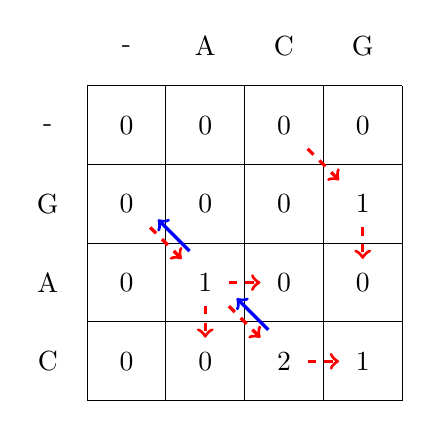
\begin{tikzpicture}[set style={{help lines}+=[dashed]}, xscale=1.0, yscale=1]

\draw (1,0) grid +(4,4);

\node  at  (0.5, 3.5) {-};
\node  at  (0.5, 2.5) {G};
\node  at  (0.5, 1.5) {A};
\node  at  (0.5, 0.5) {C};
\node  at  (1.5, 4.5) {-};
\node  at  (2.5, 4.5) {A};
\node  at  (3.5, 4.5) {C};
\node  at  (4.5, 4.5) {G};


\node  at  (1.5, 3.5) {0};
\node  at  (1.5, 2.5) {0};
\node  at  (1.5, 1.5) {0};
\node  at  (1.5, 0.5) {0};
\node  at  (2.5, 3.5) {0};
\node  at  (3.5, 3.5) {0};
\node  at  (4.5, 3.5) {0};

\node  at  (2.5, 2.5) {0};
\node  at  (3.5, 2.5) {0};

\draw   [red,very thick,dashed,->]   (3.8,3.2) -- (4.2,2.8);
%\draw   [red,very thick,dashed,->]   (3.8,2.5) -- (4.2,2.5);
%\draw   [red,very thick,dashed,->]   (4.5,3.2) -- (4.5,2.8);
\node  at  (4.5, 2.5) {1};

% Second row
\draw   [red,very thick,dashed,->]   (1.8,2.2) -- (2.2,1.8);
\node  at  (2.5, 1.5) {1};
\draw   [red,very thick,dashed,->]   (2.8,1.5) -- (3.2,1.5);
\node  at  (3.5, 1.5) {0};
%\draw   [red,very thick,dashed,->]   (3.8,1.5) -- (4.2,1.5);
\draw   [red,very thick,dashed,->]   (4.5,2.2) -- (4.5,1.8);
\node  at  (4.5, 1.5) {0};

% Third row
%\draw   [red,very thick,dashed,->]   (1.8,1.2) -- (2.2,0.8);
\draw   [red,very thick,dashed,->]   (2.5,1.2) -- (2.5,0.8);
\node  at  (2.5, 0.5) {0};
\draw   [red,very thick,dashed,->]   (2.8,1.2) -- (3.2,0.8);
%\draw   [red,very thick,dashed,->]   (3.5,1.2) -- (3.5,0.8);
\node  at  (3.5, 0.5) {2};
%\draw   [red,very thick,dashed,->]   (3.8,1.2) -- (4.2,0.8);
%\draw   [red,very thick,dashed,->]   (4.5,1.2) -- (4.5,0.8);
\draw   [red,very thick,dashed,->]   (3.8,0.5) -- (4.2,0.5);
\node  at  (4.5, 0.5) {1};

%\draw   [blue,very thick,<-]   (1.6,3.2) -- (1.6,2.8);
\draw   [blue,very thick,<-]   (1.9,2.3) -- (2.3,1.9);
\draw   [blue,very thick,<-]   (2.9,1.3) -- (3.3,0.9);
%\draw   [blue,very thick,<-]   (3.8,0.6) -- (4.2,0.6);


% -------- Fill numbers -----------
\end{tikzpicture} 

\column{0.6\textwidth}

Optimal score given by $\displaystyle \max_{i,j}S_{i,j}=2$.\\[2ex]

An optimal alignment can be found by \textcolor{blue}{back tracing} (C,C), (A,A) i.e.\\[2ex]
{\verb GAC\\
  AC}
\end{columns}

\end{frame}

%------------------------------------------------
\begin{frame}
\frametitle{Semi-global alignment}
Given two sequences $a_1,\ldots,a_N$ and $b_1,\ldots,b_M$, a scoring function d(x,y), we can find an optimal {\em semi-global} alignment by investigating the dynamic programming matrix of size (N+1,M+1), defined by

\begin{columns}

\column{0.6\textwidth}

\begin{align*}
 S_{0,0} =& 0, \\
S_{i,0} =& 0 \ \textrm{for all}\ i, \\
S_{0,j} =& 0 \ \textrm{for all}\ j 
\end{align*}
\[ S_{i,j}=\max
\begin{cases}
   S_{i-1,j-1} & + d(a_i,b_j)\\
   S_{i-1,j} & + d(a_i,-)\\
   S_{i,j-1} & + d(-,b_j)
\end{cases}
\]

\column{0.4\textwidth}

The score of an optimal alignment is $\displaystyle \max(\max_{i}S_{i,M},\max_{j}S_{N,j})$


\end{columns}

\end{frame}

%------------------------------------------------
\begin{frame}
\frametitle{The matrix representation of an alignment}
\begin{columns}

\column{0.6\textwidth}
If your alignment is in position $a_i,b_j$ witch you for the examples sake reached by a match, then the next step in the alignment is either a {\color{green}match} between  $a_{i+1},b_{j+1}$ (diagonal movement):

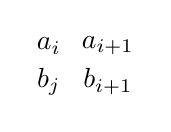
\begin{tikzpicture}[set style={{help lines}+=[dashed]}, xscale=0.75, yscale=0.45]
\draw (0,0) grid +(0,0);
\node  at  (-0.5, 1.5) {$a_{i}$};
\node  at  (-0.5, 0.5) {$b_{j}$};
\node  at  (0.5, 1.5) {$a_{i+1}$};
\node  at  (0.5, 0.5) {$b_{i+1}$};
\end{tikzpicture} 

A {\color{magenta}delete}, (a vertical movement):

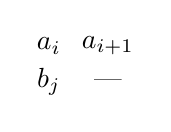
\begin{tikzpicture}[set style={{help lines}+=[dashed]}, xscale=0.75, yscale=0.45]
\draw (0,0) grid +(0,0);
\node  at  (-0.5, 1.5) {$a_{i}$};
\node  at  (-0.5, 0.5) {$b_{j}$};
\node  at  (0.5, 1.5) {$a_{i+1}$};
\node  at  (0.5, 0.5) {---};
\end{tikzpicture} 

An {\color{orange}insert}, (a horizontal movement):

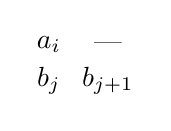
\begin{tikzpicture}[set style={{help lines}+=[dashed]}, xscale=0.75, yscale=0.45]
\draw (0,0) grid +(0,0);
\node  at  (-0.5, 1.5) {$a_{i}$};
\node  at  (-0.5, 0.5) {$b_{j}$};
\node  at  (0.5, 1.5) {---};
\node  at  (0.5, 0.5) {$b_{j+1}$};
\end{tikzpicture} 

\column{0.4\textwidth}
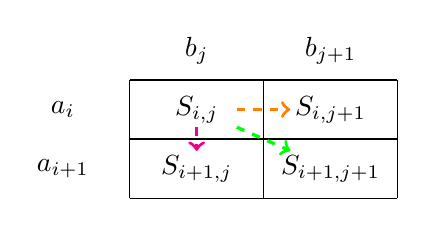
\begin{tikzpicture}[set style={{help lines}+=[dashed]}, xscale=1.7, yscale=0.75]

\draw (0,0) grid +(2,2);

\node  at  (-0.5, 1.5) {$a_{i}$};
\node  at  (-0.5, 0.5) {$a_{i+1}$};
\node  at  (0.5, 2.5) {$b_{j}$};
\node  at  (1.5, 2.5) {$b_{j+1}$};
\node  at  (0.5, 1.5) {$S_{i,j}$};
\node  at  (1.5, 0.5) {$S_{i+1,j+1}$};
\node  at  (0.5, 0.5) {$S_{i+1,j}$};
\node  at  (1.5, 1.5) {$S_{i,j+1}$};
\draw   [green,very thick,dashed,->]   (0.8,1.2) -- (1.2,0.8);
\draw   [magenta,very thick,dashed,->]   (0.5,1.2) -- (0.5,0.8);
\draw   [orange,very thick,dashed,->]   (0.8,1.5) -- (1.2,1.5);

% -------- Fill numbers -----------
\end{tikzpicture} 

\end{columns}

\end{frame}
%------------------------------------------------
\begin{frame}
\frametitle{Matrix representation of an alignment}
\begin{columns}

\column{0.6\textwidth}

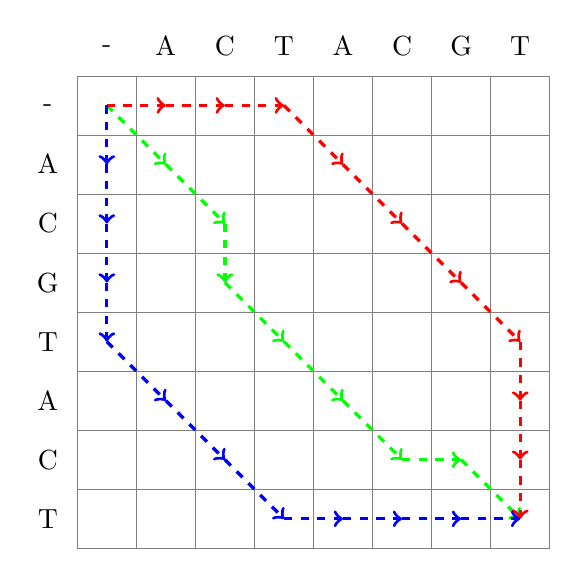
\begin{tikzpicture}[set style={{help lines}+=[dashed]}, xscale=0.75, yscale=0.75]
% Grid
\draw[step=1cm,gray,very thin] (0,-1) grid (8,7);

% Labels for ACTACT
\node at (-0.5, 6.5) {-};
\node at (-0.5, 5.5) {A};
\node at (-0.5, 4.5) {C};
\node at (-0.5, 3.5) {G};
\node at (-0.5, 2.5) {T};
\node at (-0.5, 1.5) {A};
\node at (-0.5, 0.5) {C};
\node at (-0.5, -0.5) {T};

% Labels for ACTACGT
\node at (0.5, 7.5) {-};
\node at (1.5, 7.5) {A};
\node at (2.5, 7.5) {C};
\node at (3.5, 7.5) {T};
\node at (4.5, 7.5) {A};
\node at (5.5, 7.5) {C};
\node at (6.5, 7.5) {G};
\node at (7.5, 7.5) {T};

% First alignment
\draw[green, very thick, dashed, ->] (0.5,6.5) -- (1.5,5.5);  % A -> A
\draw[green, very thick, dashed, ->] (1.5,5.5) -- (2.5,4.5);  % C -> C
\draw[green, very thick, dashed, ->] (2.5,4.5) -- (2.5,3.5);  % % Gap in first sequence (after C)
\draw[green, very thick, dashed, ->] (2.5,3.5) -- (3.5,2.5);  % T -> T
\draw[green, very thick, dashed, ->] (3.5,2.5) -- (4.5,1.5);  % A -> A
\draw[green, very thick, dashed, ->] (4.5,1.5) -- (5.5,0.5);  % C -> C
\draw[green, very thick, dashed, ->] (5.5,0.5) -- (6.5,0.5);  % Gap in second sequence (before T)
\draw[green, very thick, dashed, ->] (6.5,0.5) -- (7.5,-0.5);  % T -> T

% Second alignment
\draw[red, very thick, dashed, ->] (0.5,6.5) -- (1.5,6.5);  % insert
\draw[red, very thick, dashed, ->] (1.5,6.5) -- (2.5,6.5);  % insert
\draw[red, very thick, dashed, ->] (2.5,6.5) -- (3.5,6.5);  % insert
\draw[red, very thick, dashed, ->] (3.5,6.5) -- (4.5,5.5);  % A -> A
\draw[red, very thick, dashed, ->] (4.5,5.5) -- (5.5,4.5);  % C -> C
\draw[red, very thick, dashed, ->] (5.5,4.5) -- (6.5,3.5);  % G -> G
\draw[red, very thick, dashed, ->] (6.5,3.5) -- (7.5,2.5);  % T -> T
\draw[red, very thick, dashed, ->] (7.5,2.5) -- (7.5,1.5);  % delete
\draw[red, very thick, dashed, ->] (7.5,1.5) -- (7.5,0.5);  % delete
\draw[red, very thick, dashed, ->] (7.5,0.5) -- (7.5,-0.5);  % delete

% Third alignment
\draw[blue, very thick, dashed, ->] (0.5,6.5) -- (0.5,5.5);  % delete
\draw[blue, very thick, dashed, ->] (0.5,5.5) -- (0.5,4.5);  % delete
\draw[blue, very thick, dashed, ->] (0.5,4.5) -- (0.5,3.5);  % delete
\draw[blue, very thick, dashed, ->] (0.5,3.5) -- (0.5,2.5);  % delete
\draw[blue, very thick, dashed, ->] (0.5,2.5) -- (1.5,1.5);  % 
\draw[blue, very thick, dashed, ->] (1.5,1.5) -- (2.5,0.5);  % 
\draw[blue, very thick, dashed, ->] (2.5,0.5) -- (3.5,-0.5);  % 
\draw[blue, very thick, dashed, ->] (3.5,-0.5) -- (4.5,-0.5);  % insert
\draw[blue, very thick, dashed, ->] (4.5,-0.5) -- (5.5,-0.5);  % insert
\draw[blue, very thick, dashed, ->] (5.5,-0.5) -- (6.5,-0.5);  % insert
\draw[blue, very thick, dashed, ->] (6.5,-0.5) -- (7.5,-0.5);  % insert


\end{tikzpicture}


\column{0.4\textwidth}

\color{red}
\verb ---ACGTACT \\
\verb ACTACGT--- \\[2em]

\color{green}
\verb ACGTAC-T\\
\verb AC-TACGT\\[2em]

\color{blue}
\verb ACGTACT----\\
\verb ----ACTACGT


\end{columns}


\end{frame}


%------------------------------------------------
\begin{frame}
\begin{columns}
\column{37em}
\vspace{1cm}
\Huge{\centerline{\usebeamercolor[fg]{title}Thanks!}}
\end{columns}
\end{frame}

\end{document}
